



\subsection{Body-Centric vs Inertial Representation}

In robotics or computer vision, we are typically concerned with rotations
so that we can describe the movement of physical objects. When we
do this, it turns out that choice of coordinate frame also introduces
some interesting consequences that may or may not be intentional.
Rotational dynamics of any arbitrary coordinate frame $j$ with respect
to another coordinate frame $i$ is given by

\[
\dot{R}_{i}^{j}=R_{i}^{j}\skew{\omegabf_{i/j}^{i}}.
\]
However, let's study a concrete example: the dynamics of some rigid
body undergoing pure rotation. If we define some inertial frame $I$
and the moving, body frame as $b$, then the dynamics of the \emph{body-centric}
rotation matrix (i.e. body$\to$inertial), we get 

\begin{equation}
\dot{R}_{b}^{I}=R_{b}^{I}\skew{\omegabf_{b/I}^{b}},\label{eq:body_rot_dyn}
\end{equation}
and the \emph{inertial} rotation matrix is (inertial$\to$body) evolves
according to

\begin{equation}
\dot{R}_{I}^{b}=R_{I}^{b}\skew{\omegabf_{I/b}^{I}}.\label{eq:inertial_rotation_dynamics}
\end{equation}
This is all fine, except that we typically measure angular velocity
in the body coordinate frame $\omegabf_{b/I}^{b}.$ Therefore, it is much
more convenient to express Eq. \ref{eq:inertial_rotation_dynamics}
in terms of body angular rates. If we do this, then we get

\begin{align*}
\dot{R}_{I}^{b} & =R_{I}^{b}\skew{-R_{b}^{I}\omegabf_{b/I}^{b}} & \grey{\text{(Negate and rotate \ensuremath{\w})}}\\
 & =-\skew{\omegabf_{b/I}^{b}}R_{I}^{b}, & \grey{\text{(Eq. \ref{eq:skew_trick_2})}}
\end{align*}
which can also be easily derived as the transpose of Eq \ref{eq:body_rot_dyn}.
The desire to express our angular rates in terms of the body frame
induces a similar effect in unit quaternion dynamics, except that
it is reversed due to the reversed order of concatenation:

\begin{align}
\dot{\qbf}_{I}^{b} & =\frac{1}{2}\qbf_{I}^{b}\cdot\begin{pmatrix}0\\
\omegabf_{b/I}^{b}
\end{pmatrix}\label{eq:quaternion_dynamics}\\
\dot{\qbf}_{b}^{I} & =-\frac{1}{2}\begin{pmatrix}0\\
\omegabf_{b/I}^{b}
\end{pmatrix}\cdot\qbf_{b}^{I}.\nonumber 
\end{align}

Any advantage to expressing attitude in body-centric vs. inertial
coordinates will be use-case specific, so both representations are
used widely in literature. Because both representations are often
used, however, it can sometimes be confusing to compare two works
which may be expressing their attitude differently, especially if
neither work is specific about their representation.

\subsection{Right vs. Left Invariance of Rotation Dynamics}

Another non-trivial consequence of differing attitude representations
is whether the kinematics are left or right-invariant (LI or RI).
Body-centric rotation kinematics are left-invariant. This means that
if we have some constant matrix $A\in\SO\left(3\right)$, and we multiply
the kinematics (Eq. \ref{eq:body_rot_dyn}) by $A$ on the left, we
get a new differential equation with the same form as Eq. \ref{eq:body_rot_dyn}.

\[
\frac{d}{dt}\left(AR_{b}^{I}\right)=AR_{b}^{I}\skew{\omegabf_{b/I}^{b}}
\]
One can see that we do not get a differential equation of the same
form if we multiply both sides of Eq. \ref{eq:body_rot_dyn} on the
\emph{right} by $A.$

Inertial rotation kinematics, on the other hand, are right-invariant.
If we multiply both sides of Eq. \ref{eq:inertial_rotation_dynamics}
on the right by $A$, we get

\[
\frac{d}{dt}\left(R_{I}^{b}A\right)=-\skew{\omegabf_{b/I}^{b}}R_{I}^{b}A,
\]
which has the same form as Eq. \ref{eq:inertial_rotation_dynamics}.
A similar effect can be observed in quaternion dynamics, but with
the order reversed.

The left-right invariance shows up because of our choice in representing
$\w$ in the body frame. I know this is jumping ahead a bit, but the
Adjoint representation will allow us to flip back and forth between
left- and right-vectors as necessary, making this distinction also
a matter of convenience.

\subsection{The Solution to the Rotational Dynamics Equation}

Equations \ref{eq:body_rot_dyn} and \ref{eq:inertial_rotation_dynamics}
are first-order matrix differential equations. These are solved with
the matrix exponential we discussed in Section \ref{sec:mat_exp}.
The solution to the body-centric equation is

\[
R_{b}^{I}\left(t\right)=R_{b}^{I}\left(t_{0}\right)\exp\left(\skew{\omegabf_{b/I}^{b}}t\right)
\]
and the inertial dynamics are solved with

\[
R_{I}^{b}\left(t\right)=\exp\left(-\skew{\omegabf_{b/I}^{b}}t\right)R_{I}^{b}\left(t_{0}\right).
\]
Quaternion dynamics are also easily solved in a similar fashion, as
in

\begin{align*}
\qbf_{b}^{I}\left(t\right) & =\exp\begin{pmatrix}0\\
-\omegabf_{b/I}^{b}t
\end{pmatrix}\cdot\qbf_{b}^{I}\left(t_{0}\right)\\
\qbf_{I}^{b}\left(t\right) & =\qbf_{I}^{b}\left(t_{0}\right)\cdot\exp\begin{pmatrix}0\\
\omegabf_{b/I}^{b}t
\end{pmatrix}.
\end{align*}
The infinite series Eq. \ref{eq:mat_exp_inf} can be used to compute
these directly. However, efficient closed-form implementations are
derived in Section \ref{sec:matrix_exp_closed_form}.

\section{Transformations}

Now we venture into the world of rigid body transformations. These
allow us to represent both translation and rotation simultaneously.
As with rotations, there are two popular representations that I will
consider in this document, the first is matrix-based, the set of $4\times4$
matrices, commonly known as $\SE\left(3\right)$. The second (like
rotations) will be based on complex numbers, dual unit quaternions.
There are actually other representations, but we will see later all
of these groups share the same Lie Algebra! Therefore, we can choose
the representation that we feel most comfortable with, or is the most
efficient, etc... It really doesn't matter, which is a great thing.

\subsection{Homogeneous Transform Matrices}

Homogeneous transforms take the form of $4\times4$ matrices. These
are members of the Special Euclidean group of 3 dimensions, or $\SE\left(3\right)$.
This is by far the most common representation in robotics; it's efficient,
and the Lie group/Lie algebra is probably the most straight-forward.
A homogeneous transform matrix has the following block structure:

\[
T_{a}^{b}=\begin{bmatrix}R_{a}^{b} & \t_{b/a}^{a}\\
0 & 1
\end{bmatrix},
\]
where you have the rotation matrix in the upper left corner and the
translation vector in the third column.

Let's walk through in a block-wise format what happens when two transforms
are multiplied together. All we need to do is follow the matrix multiplication
rules and see how the coordinate frames work out. I found this to
be a very useful exercise when I first got started. It really hit
home to me how the matrices concatenate in the same way as rotation
matrices, and the potentially confusing parameterization of the translation
vector. This procedure looks like the this:

\begin{align*}
T_{a}^{c} & =T_{b}^{c}\cdot T_{a}^{b}\\
 & =\begin{bmatrix}R_{b}^{c} & \t_{c/b}^{c}\\
0 & 1
\end{bmatrix}\cdot\begin{bmatrix}R_{a}^{b} & \t_{b/a}^{b}\\
0 & 1
\end{bmatrix}\\
 & =\begin{bmatrix}R_{b}^{c}R_{a}^{b} & R_{b}^{c}\t_{b/a}^{b}+\t_{c/b}^{c}\\
0 & 1
\end{bmatrix}\\
 & =\begin{bmatrix}R_{a}^{c} & \t_{c/a}^{c}\\
0 & 1
\end{bmatrix}.
\end{align*}
So we see, we get what we expect: all the coordinate frames land the
way we want.

We can also perform the same exercise for taking the inverse. Remember
that the inverse of a matrix is $\nicefrac{1}{\det\left(A\right)\textrm{Adj\ensuremath{\left(A\right)}}}$,
where Adj$\left(A\right)$ refers to the adjugate of $A.$ Because
it gets a little nasty, I'm going to skip actually computing the adjugate,
but if you work it out, you can see how this apparently super convenient
result just pops out:

\begin{align*}
\left(T_{a}^{b}\right)^{-1} & =\begin{bmatrix}R_{a}^{b} & \t_{b/a}^{b}\\
0 & 1
\end{bmatrix}^{-1}\\
 & =\frac{1}{\det\left(T_{a}^{b}\right)}\textrm{Adj}\left(T_{a}^{b}\right)\\
 & =\frac{1}{1}\begin{bmatrix}\left(R_{a}^{b}\right)^{\top} & -\left(R_{a}^{b}\right)^{\top}\t_{b/a}^{b}\\
0 & 1
\end{bmatrix}\\
 & =\begin{bmatrix}R_{b}^{a} & -R_{b}^{a}\t_{b/a}^{b}\\
0 & 1
\end{bmatrix}\\
 & =\begin{bmatrix}R_{b}^{a} & \t_{a/b}^{a}\\
0 & 1
\end{bmatrix}\\
 & =T_{b}^{a}.
\end{align*}
Boom. 

If you didn't notice, it's really important to note is that the translation
vector is defined in the \emph{destination} frame, rather than the
origin frame of the rotation matrix. This isn't a problem, but it
was very confusing for me at first.

\subsection{Passive and Active Transformations}

The same notion of passive and active transformations discussed with
rotations applies here. To perform a passive transformation with $\SE\left(3\right)$,
we just pad the vector to be rotated with an extra $1$ at the bottom,
and multiply by our transform matrix. Just for completeness, let us
walk through what happens when we do this in a block-wise format

\begin{align*}
\rbf_{b/p}^{b} & =T_{a}^{b}\cdot\rbf_{a/p}^{a}\\
 & =\begin{bmatrix}R_{a}^{b} & \t_{b/a}^{b}\\
0 & 1
\end{bmatrix}\cdot\begin{bmatrix}\rbf_{a/p}^{a}\\
1
\end{bmatrix}\\
 & =\begin{bmatrix}R_{a}^{b}\rbf_{a/p}^{a}+\t_{b/a}^{b}\\
1
\end{bmatrix}\\
 & =\rbf_{b/p}^{b}.
\end{align*}
Doing this at least once is another exercise that I found to be very
helpful when first trying to use $\SE\left(3\right).$ 

\begin{figure}[H]
\begin{centering}
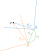
\includegraphics[width=0.3\columnwidth]{chap2_preliminaries/figures/transform_passive}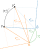
\includegraphics[width=0.3\columnwidth]{chap2_preliminaries/figures/transform_active}
\par\end{centering}
\caption{Illustration of a passive transformation (left) and an active transformation
(right)}
\label{fig:passive_transform}
\end{figure}

An active transformation occurs by multiplying by the inverse of the
passive transform as shown in Figure \ref{fig:passive_transform}.
Just as with rotations, If you walk through the coordinate frames
of an active transformation, you'll see that the coordinate frames
don't line up right in our notation. This is because the active transformation
does not preserve the location. Instead we have defined a new location,
based on the coordinates of $p$ in frame $a$ projected into frame
$b$. I have tried to represent this with the $p^{\star}$ notation
in Figure \ref{fig:passive_transform}.

Transform matrices are an obvious extension to rotation matrices.
However, just like rotation matrices, the complex number representation
is more efficient. This brings us to our next transform parameterization:
dual unit quaternions.

\subsection{Dual Unit Quaternions}

The use of dual unit quaternions is another approach to representing
a rigid body transform that relies on complex numbers. As one might
expect, it can also be considered as two copies of $\SU\left(2\right)$
as well. Dual quaternions are more popular in the computer graphics
and physics community, and for the same reasons that quaternions often
out-perform rotation matrices, dual quaternions are often yield the
most efficient representation for rigid body transformations.

Before I jump into dual quaternions, I'm going to first introduce
dual numbers. Dual numbers are similar in many ways to imaginary numbers.
The idea is that we define a scalar $\epsilon$ as a mathematical
construct that splits a numerical representation into two components.
For example, we might have the dual number 
\[
z=r+d\epsilon,
\]
where $r$ is the real part, and $d$ is the dual part. We also define
$\epsilon$ as having special rules where $\epsilon^{2}=0,$ but $\epsilon\neq0.$
Again, this is similar to complex numbers where we use $i$ to distinguish
imaginary components from real components. The dual operator $\epsilon$
is used in much the same way. It should be noted that $\epsilon$
in this context is just a special symbol. It is \emph{not} related
to small perturbations, as it is used in other areas of mathematics.
Trying to interpret it in this way can sometimes be confusing.

Dual numbers follow these basic rules. If two dual numbers are added,
then the real part and dual part are simply summed separately (just
like imaginary numbers). For example,

\[
x=a+b\epsilon,\quad y=c+d\epsilon
\]

\[
x+y=\left(a+c\right)+\left(b+d\right)\epsilon.
\]
Multiplication also is performed similarly to complex multiplication,
but with the rule that $\epsilon^{2}=0$. For example,

\begin{align*}
x\cdot y & =ac+ad\epsilon+bc\epsilon+bd\epsilon^{2}\\
 & =ac+\left(ad+bc\right)\epsilon.
\end{align*}
Finally, dual variables have their own concept of conjugate, given
in the expected way and denoted as $\left(\cdot\right)^{*}.$ For
example,
\begin{align*}
z & =r+d\epsilon\\
z^{*} & =r-d\epsilon.
\end{align*}
If $r$ and $d$ are also complex variables, then we actually have
three forms of conjugation. Imaginary conjugation, dual conjugation,
and imaginary-dual conjugation, given as

\begin{align*}
\bar{z} & =\bar{r}+\bar{d}\epsilon & \text{imag}\\
z^{*} & =r-d\epsilon. & \text{dual}\\
\bar{z}^{*} & =\bar{r}-\bar{d}\epsilon. & \text{imag+dual}
\end{align*}

Now we are ready to talk about dual quaternions, $\mathbb{D}\S^{3}$
and $\mathbb{D}\SU\left(2\right)$\footnote{The $\mathbb{D}$ here refers to the dual formulation.}.
We can represent 3D transforms with the dual unit quaternion pair

\[
\qq=\qbf_{r}+\epsilon\qbf_{d},
\]
where $\qbf_{r}$ is called the real part and $\qbf_{d}$ is the dual
part. The real part contains the rotation, while the dual part is
one-half the pure quaternion containing the translation half rotated,
as in\footnote{This may seem like a weird parameterization, and some (like myself)
may question if there is a simpler way, rather than handling this
half-rotated vector. It comes from using the simplest form of the
underlying Lie Algebra, and finding the natural expression of that
group in dual quaternions. Trying to form a convenient group and mangling
the underlying algebra to match results in losing a lot of the beauty
of Lie Theory. It's better to just use the natural expression, starting
at the algebra and working up.}

\begin{align*}
\qbf_{r} & =\qbf_{a}^{b}\\
\qbf_{d} & =\frac{1}{2}\begin{pmatrix}0\\
\t_{b/a}^{a}
\end{pmatrix}\cdot\qbf_{a}^{b}.
\end{align*}
If we combine the quaternion algebra operations with the dual number,
we get dual quaternion arithmetic. Dual quaternion multiplication
is given as one might expect, with

\[
\qq_{1}\circ\qq_{2}=\qbf_{1r}\cdot\qbf_{2r}+\left(\qbf_{1r}\cdot\qbf_{2d}+\qbf_{1d}\cdot\qbf_{2r}\right)\epsilon.
\]
Let's walk through this together and make sure the coordinate frames
all line up. Before we do this, however, we need the following trick.
If we take the quaternion rotation formula, and split it up, we get
an expression for dealing with half-rotated vectors:

\begin{align}
\t^{b} & =\left(\qbf_{a}^{b}\right)^{-1}\cdot\t^{a}\cdot\qbf_{a}^{b}\nonumber \\
\qbf_{a}^{b}\cdot\t^{b} & =\qbf_{a}^{b}\cdot\left(\qbf_{a}^{b}\right)^{-1}\cdot\t^{a}\cdot\qbf_{a}^{b}\nonumber \\
\qbf_{a}^{b}\cdot\t^{b} & =\t^{a}\cdot\qbf_{a}^{b}.\label{eq:quat_switch_trick}
\end{align}
Now can work through the dual quaternion arithmetic, and see how dual
quaternion multiplication results in concatenating transforms.

\begin{align*}
\qq_{a}^{b}\circ\qq_{b}^{c} & =\qbf_{a}^{b}\cdot\qbf_{b}^{c}+\frac{\epsilon}{2}\left(\qbf_{a}^{b}\cdot\begin{pmatrix}0\\
\t_{c/b}^{b}
\end{pmatrix}\cdot\qbf_{b}^{c}+\begin{pmatrix}0\\
\t_{b/a}^{a}
\end{pmatrix}\cdot\qbf_{a}^{b}\cdot\qbf_{b}^{c}\right)\\
 & =\qbf_{a}^{c}+\frac{\epsilon}{2}\left(\begin{pmatrix}0\\
\t_{c/b}^{a}
\end{pmatrix}\cdot\qbf_{a}^{b}\cdot\qbf_{b}^{c}+\begin{pmatrix}0\\
\t_{b/a}^{a}
\end{pmatrix}\cdot\qbf_{a}^{b}\cdot\qbf_{b}^{c}\right) & \grey{\textrm{(Eq. \ref{eq:quat_switch_trick})}}\\
 & =\qbf_{a}^{c}+\frac{\epsilon}{2}\left(\begin{pmatrix}0\\
\t_{c/a}^{a}
\end{pmatrix}\cdot\qbf_{a}^{c}\right).
\end{align*}

Inverting (or computing the complex conjugate of) a dual quaternion
is as simple as inverting the two components. To work through this
operation, line by line, we will also need to use the trick from Eq.
\ref{eq:quat_switch_trick}.

\begin{align*}
\left(\qbfq_{a}^{b}\right)^{-1} & =\left(\qbf_{a}^{b}\right)^{-1}+\frac{\epsilon}{2}\left(\begin{pmatrix}0\\
\t_{b/a}^{a}
\end{pmatrix}\cdot\qbf_{a}^{b}\right)^{-1}\\
 & =\qbf_{b}^{a}+\frac{\epsilon}{2}\left(\left(\qbf_{a}^{b}\right)^{-1}\cdot\begin{pmatrix}0\\
\t_{b/a}^{a}
\end{pmatrix}^{-1}\right)\\
 & =\qbf_{b}^{a}+\frac{\epsilon}{2}\left(\qbf_{b}^{a}\cdot\begin{pmatrix}0\\
\t_{a/b}^{a}
\end{pmatrix}\right)\\
 & =\qbf_{b}^{a}+\frac{\epsilon}{2}\left(\begin{pmatrix}0\\
\t_{a/b}^{b}
\end{pmatrix}\cdot\qbf_{b}^{a}\right) & \textrm{\ensuremath{\grey{\textrm{(Eq. \ref{eq:quat_switch_trick})}}}}\\
 & =\qq_{b}^{a}
\end{align*}

Transforming a vector is done by creating a pure quaternion (with
no rotational component) from the translation vector, then pre- and
post-multiplying by the dual quaternion and its dual-complex conjugate.
If we work through the steps we can see how this works:

\begin{align*}
\rbf_{p/b}^{b} & =\left(\bar{\qq_{a}^{b}}\right)^{*}\circ\rbf_{p/a}^{a}\circ\qq_{a}^{b}\\
 & =\left[\qbf_{b}^{a}-\frac{\epsilon}{2}\left(\t_{a/b}^{b}\cdot\qbf_{b}^{a}\right)\right]\circ\left[\boldsymbol{1}+\epsilon\rbf_{p/a}^{a}\right]\circ\left[\qbf_{a}^{b}+\frac{\epsilon}{2}\left(\t_{b/a}^{a}\cdot\qbf_{a}^{b}\right)\right]\\
 & =\left[\qbf_{b}^{a}-\frac{\epsilon}{2}\left(\t_{a/b}^{b}\cdot\qbf_{b}^{a}\right)\right]\circ\left[\left(\boldsymbol{1}\cdot\qbf_{a}^{b}\right)+\frac{\epsilon}{2}\left(\boldsymbol{1}\cdot\left(\t_{b/a}^{a}\cdot\qbf_{a}^{b}\right)+2\rbf_{p/a}^{a}\cdot\qbf_{a}^{b}\right)\right]\\
 & =\left(\qbf_{b}^{a}\cdot\qbf_{a}^{b}\right)+\frac{\epsilon}{2}\left(\qbf_{b}^{a}\cdot\left(\left(-\t_{b/a}^{a}\cdot\qbf_{a}^{b}\right)+2\rbf_{p/a}^{a}\cdot\qbf_{a}^{b}\right)+\left(\t_{a/b}^{b}\cdot\qbf_{b}^{a}\right)\cdot\qbf_{a}^{b}\right)\\
 & =\boldsymbol{1}+\frac{\epsilon}{2}\left(\qbf_{b}^{a}\cdot\left(-\t_{b/a}^{a}\cdot\qbf_{a}^{b}\right)+\qbf_{b}^{a}\cdot2\rbf_{p/a}^{a}\cdot\qbf_{a}^{b}+\left(\t_{a/b}^{b}\cdot\qbf_{b}^{a}\right)\cdot\qbf_{a}^{b}\right)\\
 & =\boldsymbol{1}+\frac{\epsilon}{2}\left(-\t_{b/a}^{b}+2\rbf_{p/a}^{b}+\t_{a/b}^{b}\right)\\
 & =\boldsymbol{1}+\frac{\epsilon}{2}\left(2\rbf_{p/a}^{b}-2\t_{b/a}^{b}\right)\\
 & =\boldsymbol{1}+\epsilon\left(\rbf_{p/b}^{b}\right).
\end{align*}


\subsection{Dynamics and Invariance}

As with rotations, the same concept of left- and right-invariance
also applies to transforms. If we parameterize rigid body dynamics
in body-centric coordinates, we get the left-invariant dynamics

\[
\dot{T}_{b}^{I}=T_{b}^{I}\begin{pmatrix}\skew{\omegabf_{b/I}^{b}} & \v_{b/I}^{b}\\
0 & 1
\end{pmatrix}.
\]
and the inertial coordinates have right-invariant dynamics, given
as

\[
\dot{T}_{I}^{b}=\begin{pmatrix}-\skew{\omegabf_{b/I}^{b}} & -\v_{b/I}^{b}\\
0 & 1
\end{pmatrix}T_{I}^{b}
\]
Like ordinary quaternions and rotation matrices, dual quaternions
also concatenate opposite $\SE\left(3\right)$, so the order of the
dynamic equations is flipped, as in

\begin{align*}
\dot{\qq}_{b}^{I} & =-\frac{1}{2}\left(\begin{pmatrix}0\\
\omegabf_{b/I}^{b}
\end{pmatrix}+\epsilon\begin{pmatrix}0\\
\v_{b/I}^{b}
\end{pmatrix}\right)\circ\qq_{b}^{I}\left(t_{0}\right)\\
\dot{\qq}_{I}^{b} & =\frac{1}{2}\qq_{I}^{b}\circ\left(\begin{pmatrix}0\\
\omegabf_{b/I}^{b}
\end{pmatrix}+\epsilon\begin{pmatrix}0\\
\v_{b/I}^{b}
\end{pmatrix}\right).
\end{align*}


\section{Lie Groups}

Lie Group theory is a very old discipline deeply rooted in mathematics
and theoretical physics. It was developed to better understand and
model nature at the most fundamental levels. In fact, much of particle
physics can be modeled using Lie group theory, including special relativity
and quantum dynamics. While we don't often need to properly model
Minkowski space, we can learn a lot about modeling physical systems
by piggybacking on physics literature.

If you can't tell from the last 4 sections, we end up doing a lot
of reasoning about coordinate frames in robotics. We often need to
reason about how they move, and how they relate to one another. We
also find ourselves trying to infer things about these coordinate
frames given noisy sensor measurements. There are a variety of ways
that we could do this, but the real problems show up when we need
to this in real time under realistic computational limitations. 

To meet actual computational requirements, we generally want to be
able to leverage linear algebra and all of its tools. Unfortunately,
however, coordinate frame transformations are not vectors, so it's
not completely obvious how we can use these tools in a principled
manner. Luckily, we have Lie group theory that can bridge this gap.
We will see in this section how we can use Lie Groups to take non-vector
group objects, and map them into a vector space where we can perform
linear algebra and reason about things in an efficient manner, then
map our results back into the group so we can do useful things.

As a further motivating example, consider the case where we might
want to represent our uncertainty of some estimate of a rotation matrix.
In general, assuming that our uncertainty of some vector quantity
$\x$ can be represented with a multivariate Gaussian distribution,
the covariance of this distribution is computed as

\[
\Sigma_{\x}=E\left[\left(\x-\hat{\x}\right)\left(\x-\hat{\x}\right)^{\top}\right],
\]
where $\hat{\x}$ was our best estimate and $\x$ was the true value.
However, if we consider putting our rotation matrix $R$ into this
equation, what does $R-\hat{R}$ even mean? Subtraction is not a sensible
operation when talking about rotation matrices. First off, it would
no longer be a rotation matrix, as it would not longer have unit determinant,
and second, it would have nine parameters, when we expect there to
only be three\footnote{Using Euler angles doesn't get you out of this, either. It's just
more subtle. Think about what it really means to subtract two ``vectors''
of euler angles. The intermediate axes defining the Euler angle parameterization
will not line up, so it's not a sensible operation.}. Lie group theory solves this problem for us, as we will soon find
out.

\subsection{Group Theory}

Before we launch into Lie groups, let us consider groups generically.
A group is simply a set of members which are \emph{closed} under some
group operator. This means that if I had two group members $g_{1}$
and $g_{2}$ and I act on these members with the group operator $\circ$,
then the result should also be a part of the group. For example,

\[
g_{1}\circ g_{2}=g_{3},\qquad\qquad g_{1},g_{2},g_{3}\in G.
\]
We use groups all the time, maybe without knowing it. Some commonly
used groups in robotics are vectors (closed under vector addition),
rotation matrices (closed under matrix multiplication), and quaternions
(closed under quaternion multiplication). Some more exotic groups
could include binary vectors closed under bit-wise-XOR, positive definite
matrices closed under matrix addition and integers closed under addition.\footnote{In case you need another reason to stop using Euler angles, Euler
angles aren't even a group, unless, of course, the group operator
is defined as ``convert to rotation matrix, multiply, and then convert
back to Euler angles''}

\subsection{Lie Group Definition}

A Lie group is a group that is also a differentiable manifold. What
this means is that every group element $A$ induces a map from one
group element \textbf{$B$} to another $C=A\circ B$ and that this
mapping is differentiable. Of all the groups mentioned above, vectors,
rotation matrices, quaternions and positive definite matrices are
also Lie Groups, while binary vectors closed under XOR and integers
are not, because the mappings are not differentiable.

Each Lie groups has an associated Lie algebra, typically indicated
by using the fraktur font, (i.e. $\so\left(3\right)).$ A Lie algebra
is a vector space $\mathfrak{g}$ equipped with a binary operation
called the \emph{Lie bracket,} $[,]$. For matrix Lie algebras, the
Lie bracket is given as

\[
\left[A,B\right]=AB-BA.
\]
The Lie bracket abides by the following rules:
\begin{itemize}
\item Bilinearity: $\left[aX+bY,Z\right]=a\left[X,Z\right]+b\left[Y,Z\right]$
\item Anticommutativity: $\left[X,Y\right]=-\left[Y,X\right]\quad\forall X,Y\in\mathfrak{g}$
\item The Jacobi Identity: $\left[X,\left[Y,Z\right]\right]+\left[Z,\left[X,Y\right]\right]+\left[Y,\left[Z,X\right]\right]=0\quad\forall X,Y,Z\in\mathfrak{g}$
\end{itemize}
The Lie Algebra defines something equivalent to the basis of the Lie
Group, except instead of basis vectors, we have \emph{generators}.
The generators are the building blocks of the group, and typically
encode the degrees of freedom in a orthonormal way. Each member of
any Lie Algebra can be expressed as the exponential of a linear combination
of the generators.

There is an important theorem that we will use a little later called
the Baker-Campbell-Hausdorff Theorem (BCH). This theorem states that
the solution $Z$ to

\[
e^{X}e^{Y}=e^{Z},
\]
can be expressed as a power series involving commutators $X$ and
$Y$ in the Lie bracket. The first couple terms of this series is
given as

\[
Z=X+Y+\frac{1}{2}\left[X,Y\right]+\frac{1}{12}\left[X,\left[X,Y\right]\right]-\frac{1}{12}\left[Y,\left[X,Y\right]\right]+\dots.
\]
This formula is central to many proofs in the Lie group-Lie algebra
correspondence.

\subsection{The Generators of $\protect\SO\left(3\right)$}

The easiest way to come up with the generators of a Lie Group is to
consider the infinitesimal transformations that the group can accommodate.
For example, the generators of $\so\left(3\right)$ are given by

\begin{align*}
J_{1} & =\begin{pmatrix}0 & 0 & 0\\
0 & 0 & -1\\
0 & 1 & 0
\end{pmatrix} & J_{2} & =\begin{pmatrix}0 & 0 & 1\\
0 & 0 & 0\\
-1 & 0 & 0
\end{pmatrix} & J_{3} & =\begin{pmatrix}0 & -1 & 0\\
1 & 0 & 0\\
0 & 0 & 0
\end{pmatrix}.
\end{align*}
Obviously, there is a lot more rigor here than I can really provide,
not being a mathematician myself\footnote{For example, I'm not sure if the choice to make these line up exactly
with the skew-symmetric matrix simply a matter of convenience or something
more fundamental.}. However, we can prove that these generators are correct with this
simple exercise. We know that all elements of $\SO\left(3\right)$
must follow these conditions:

\begin{align*}
A^{\top}A & =I & \det\left(A\right) & =1.
\end{align*}
We also know that every element of $\SO\left(3\right)$ can be written
in terms of some linear combination of generators $J$ as

\[
A=\exp\left(\theta J\right).
\]
We can back out the structure of $J$ through putting it into the
definition conditions of $\SO\left(3\right)$. The first condition
yields

\begin{align*}
A^{\top}A & =I\\
\exp\left(\theta J\right)^{\top}\exp\left(\theta J\right) & =I\\
J^{\top}+J & =0.
\end{align*}
If we use the second condition (and the identity $\det\left(\exp\left(A\right)\right)=\exp\left(\textrm{tr}\left(A\right)\right)$)
we see

\begin{align*}
\det\left(A\right) & =1\\
\det\left(e^{\theta J}\right) & =1\\
\textrm{tr}\left(J\right) & =0.
\end{align*}
So, the generators for the algebra $\so\left(3\right)$ must be anti-symmetric,
traceless $3\times3$ matrices. Three linearly independent matrices
fulfilling these conditions \emph{and} the rules for a lie algebra
are\footnote{Specifically, we need generators that obey the right-hand rule through
the Lie bracket so they can satisfy the Jacobi Identity.}

\begin{align*}
J_{1} & =\begin{pmatrix}0 & 0 & 0\\
0 & 0 & -1\\
0 & 1 & 0
\end{pmatrix} & J_{2} & =\begin{pmatrix}0 & 0 & 1\\
0 & 0 & 0\\
-1 & 0 & 0
\end{pmatrix} & J_{3} & =\begin{pmatrix}0 & -1 & 0\\
1 & 0 & 0\\
0 & 0 & 0
\end{pmatrix}.
\end{align*}
Therefore, these must be valid generators of $\so\left(3\right).$

As mentioned before, all members of a Lie group can be created by
computing the exponential of a linear combination of the generators.
Furthermore, because the generators are orthogonal, $\so\left(3\right)$
is isomorphic to $\R^{3}$. Therefore, to keep things concise, we
can actually form a vector whose coefficients are then multiplied
by the generators. In the case of $\SO\left(3\right)$, this is the
same as computing the skew-symmetric matrix of a vector. But in general,
the $\left(\cdot\right)^{\wedge}$ and $\left(\cdot\right)^{\vee}$
notation is used to indicate this mapping. For example, for $\so\left(3\right):$

\begin{align*}
\left(\v^{\wedge}\right) & =\sum_{i}J_{i}\e_{i}^{\top}\v\\
 & =J_{1}\v_{x}+J_{2}\v_{y}+J_{3}\v_{z}\\
 & =\begin{pmatrix}0 & -\v_{z} & \v_{y}\\
\v_{z} & 0 & -\v_{x}\\
-\v_{y} & -\v_{x} & 0
\end{pmatrix},
\end{align*}

\[
\left(\v^{\wedge}\right)^{\vee}=\v.
\]
This notation is used in some literature \cite{Barfoot2019,Sola2019},
but not in others \cite{Drummond2014,Ethan2019}. Since the two representations
(the matrix algebra and the vector) are isomorphic, the mapping to
the matrix Lie Algebra is often skipped notationally, and $\exp\left(\v\right)$
is written while $\exp\left(\v^{\wedge}\right)$ would technically
be more correct. As computing the matrix exponential of $\v\in\R^{3}$
is actually not possible given the definition above, the mapping of
the vector to the matrix Lie Algebra is implied in literature where
the mapping is ignored.

\subsection{The Generators of $\protect\SU\left(2\right)/\protect\S^{3}$}

We can follow the same procedure that we performed to derive the generators
of $\SO\left(3\right)$ to get the generators of $\SU\left(2\right)/\S^{3}$.
First, let's start with the conditions of $\SU\left(2\right)$

\[
U^{\dagger}U=UU^{\dagger}=1\qquad\qquad\det\left(U\right)=1.
\]
Now, as before, let us write these conditions in terms of the generators,
and use BCH in tandem with the fact that $\left[U^{\dagger},U\right]=0$
to get

\begin{align}
U^{\dagger}U & =1\nonumber \\
\left(\exp\left(iJ\right)\right)^{\dagger}\exp\left(iJ\right) & =1\nonumber \\
\exp\left(-iJ^{\dagger}\right)\exp\left(iJ\right) & =1\nonumber \\
\exp\left(-iJ^{\dagger}+iJ+\frac{1}{2}\text{\ensuremath{\left[J^{\dagger},J\right]}}\right)+\dots & =1 & \grey{\textrm{(BCH)}}\nonumber \\
\exp\left(-iJ^{\dagger}+iJ\right) & =1\nonumber \\
-iJ^{\dagger}+iJ & =0\nonumber \\
J^{\dagger} & =J.\label{eq:HermetianSU2}
\end{align}
Now, if we look at the second condition, (again, leveraging $\det\left(\exp\left(A\right)\right)=\exp\left(\textrm{tr}\left(A\right)\right)$),
we can see

\begin{align}
\det\left(\exp\left(iJ\right)\right) & =1\nonumber \\
\exp\left(i\textrm{tr}\left(J\right)\right) & =1\nonumber \\
\textrm{tr}\left(J\right) & =0.\label{eq:tracelessSU2}
\end{align}
So the generators must be Hermetian (Eq. \ref{eq:HermetianSU2}),
and traceless (Eq. \ref{eq:tracelessSU2}) complex $2\times2$ matrices.
The standard basis for this set is

\begin{align*}
J_{1} & =\begin{pmatrix}0 & 1\\
1 & 0
\end{pmatrix} & J_{2} & =\begin{pmatrix}0 & -i\\
i & 0
\end{pmatrix} & J_{3} & =\begin{pmatrix}1 & 0\\
0 & -1
\end{pmatrix}.
\end{align*}
This choice of generators corresponds with infinitesimal rotations
in $\SU\left(2\right),$ and because of the isomorphism between $\SU\left(2\right)$
and $\S^{3}$ (unit quaternions), we have also just derived the generators
for unit quaternions as well:

\begin{align*}
J_{1} & =i & J_{2} & =j & J_{3} & =k.
\end{align*}
This means that the $\left(\cdot\right)^{\wedge}$ operations for
$\SU\left(2\right)$ and $\S^{3}$ are given as

\[
\w^{\wedge}=\begin{pmatrix}\omegabf_{z} & \omegabf_{x}-\omegabf_{y}i\\
\omegabf_{x}+\omegabf_{y}i & \omegabf_{z}
\end{pmatrix},
\]
and

\[
\w^{\wedge}=\begin{pmatrix}0\\
\w
\end{pmatrix},
\]
respectively, while the $\left(\cdot\right)^{\vee}$operator is defined
as the inverse of either operation.

There is a very interesting relationship between $\su\left(2\right)$
and $\so\left(3\right)$. Both algebras have the following property:

\begin{align*}
\left[J_{1},J_{2}\right] & =J_{3} & \left[J_{2},J_{1}\right] & =-J_{3}\\
\left[J_{2},J_{3}\right] & =J_{1} & \left[J_{3},J_{2}\right] & =-J_{1}\\
\left[J_{3},J_{1}\right] & =J_{2} & \left[J_{1},J_{3}\right] & =-J_{2}.
\end{align*}
It turns out, this is indicative of a more fundamental result. One
can say that $\SU\left(2\right)$ and $\SO\left(3\right)$ have the
same Lie algebra, because we define Lie algebras by their Lie bracket.
Forgive the extended quotation, but this summary from \emph{Physics
From Symmetry\cite{schwichtenberg_2015}} explains this concept in
detail, as well as giving a very nice motivation for why we use Lie
Algebras in the first place.
\begin{quote}
There is precisely one simply-connected Lie group corresponding to
each Lie algebra. This simply-connected group can be thought of as
the \textquotedbl mother\textquotedbl{} of all those groups having
the same Lie algebra, because there are maps to all other groups with
the same Lie algebra from the simply connected group, but not vice
versa. We could call it the mother group of this particular Lie algebra,
but mathematicians tend to be less dramatic and call it the covering
group. All other groups having the same Lie algebra are said to be
covered by the simply connected one. $SU(2)$ is the double cover
of $SO(3)$. This means there is a two-to-one map from $SU(2)$ to
$SO(3)$.

Furthermore, $SU(2)$ is the three sphere, which is a simply connected
manifold. Therefore, we have found the \textquotedbl most important\textquotedbl{}
group belonging to the Lie algebra. We can get all other groups belonging
to this Lie algebra through maps from $SU(2)$.

We can now understand what manifold $SO(3)$ is. The map from $SU(2)$
to $SO(3)$ identifies with two points of $SU(2)$, one point of $SO(3)$.
Therefore, we can think of $SO(3)$ as the top half of $\S^{3}$

We can see, from the point of view that Lie groups are manifolds that
$SU(2)$ is a more complete object than $SO(3)$. $SO(3)$ is just
\textquotedbl part\textquotedbl{} of the complete object.

...

To describe nature at the most fundamental level, we must use the
covering group, instead of any of the other groups that one can map
to from the covering group. We are able to derive the representations
of the most fundamental group, belonging to a given Lie algebra, by
deriving representations of the Lie algebra. We can then put the matrices
representing the Lie algebra elements (the generators) into the exponential
function to get matrices representing group elements. 

Herein lies the strength of Lie theory. By using pure mathematics
we are able to reveal something fundamental about nature. The standard
symmetry group of special relativity hides something from us {[}the
spin of elementary particles{]}, because it is not the most fundamental
group belonging to this symmetry. The covering group of the Poincar�
group is the fundamental group and therefore we will use it to describe
nature.
\end{quote}
What Schwichtenberg is talking about is the fact that the double cover
of the Lorentz group is able to represent the spin of a particle,
while the standard Lorentz group cannot. This is analogous to the
difference between the use of $\S^{3}/\SU\left(2\right)$ versus $\SO\left(3\right)$.
In robotics, we are typically unconcerned with the bottom half of
the $\S^{3}$ unit sphere, so there is no fundamental drawback to
using $\SO\left(3\right)$ like there is in particle physics. However,
there is something about nature and pure mathematics that encodes
rotations in a double cover, and $\SO\left(3\right)$ only tells us
half of the story.

Finally, it's crucial to realize that the Lie groups arise from and
are defined by the Lie algebra, and therefore by the generators. Not
the other way around. By starting at the generators we can capture
at a more fundamental level what is going on in 3D rotations, and
what the manifold really is. 

\subsection{The generators of $\protect\SE\left(3\right)$}

As mentioned before, $\SE\left(3\right)$ is the set of rigid body
transforms. Lie Theory as developed by physicists has very little
to say about $\SE\left(3\right)$, as it is actually a subset of the
set of $4\times4$ matrices, known classically as the Lorentz group.
The Lorentz group (or the complexified version, octonians) are used
to encode not only rigid body transforms, but also the dilation of
space and time due to relativistic effects. In robotics, we can usually
restrict ourselves to time and space-preserving transformations, so
we can use a simplified version of the Lorentz space generators.\footnote{The bottom row of the $4\times4$ matrix is used in the Lorentz group,
whereas is it not used in $\SE\left(3\right).$ The Lorentz group
generators continue the skew-symmetric pattern we are used to in this
bottom row and right column. For more information about using Lie
groups to model spacetime, \cite{schwichtenberg_2015} is a phenomenal
introductory text to Lie groups in the context of theoretical physics.
It includes a very good explanation of the Lorentz group and its double-cover.} 

The generators of $\SE\left(3\right)$ are just the basis of infinitesimal
transformations along each degree of freedom.

\begin{align*}
J_{1} & =\begin{pmatrix}0 & 0 & 0 & 0\\
0 & 0 & -1 & 0\\
0 & 1 & 0 & 0\\
0 & 0 & 0 & 0
\end{pmatrix} & J_{2} & =\begin{pmatrix}0 & 0 & 1 & 0\\
0 & 0 & 0 & 0\\
-1 & 0 & 0 & 0\\
0 & 0 & 0 & 0
\end{pmatrix} & J_{3} & =\begin{pmatrix}0 & -1 & 0 & 0\\
1 & 0 & 0 & 0\\
0 & 0 & 0 & 0\\
0 & 0 & 0 & 0
\end{pmatrix}\\
J_{4} & =\begin{pmatrix}0 & 0 & 0 & 1\\
0 & 0 & 0 & 0\\
0 & 0 & 0 & 0\\
0 & 0 & 0 & 0
\end{pmatrix} & J_{5} & =\begin{pmatrix}0 & 0 & 0 & 0\\
0 & 0 & 0 & 1\\
0 & 0 & 0 & 0\\
0 & 0 & 0 & 0
\end{pmatrix} & J_{6} & =\begin{pmatrix}0 & 0 & 0 & 0\\
0 & 0 & 0 & 0\\
0 & 0 & 0 & 1\\
0 & 0 & 0 & 0
\end{pmatrix}.
\end{align*}
The use of these generators defines the $\left(\cdot\right)^{\wedge}$
operator for $\SE\left(3\right)$ as

\[
\begin{pmatrix}\w\\
\v
\end{pmatrix}^{\wedge}=\begin{pmatrix}\skew{\w} & \v\\
0 & 0
\end{pmatrix},
\]
and $\left(\cdot\right)^{\vee}$ as the inverse operation.

\subsection{The generators of $\mathbb{D}\protect\SU\left(2\right)$ and $\mathbb{D}\protect\S^{3}$}

As with $\SE\left(3\right),$ we use only the subset of the two copies
of $\su\left(2\right)$ necessary to encode time and space-preserving
3D transformations. The generators for this group are

\begin{align*}
J_{1} & =\begin{pmatrix}0 & 1\\
1 & 0
\end{pmatrix}+\epsilon\begin{pmatrix}0 & 0\\
0 & 0
\end{pmatrix} & J_{2} & =\begin{pmatrix}0 & -i\\
i & 0
\end{pmatrix}+\epsilon\begin{pmatrix}0 & 0\\
0 & 0
\end{pmatrix} & J_{3} & =\begin{pmatrix}1 & 0\\
0 & -1
\end{pmatrix}+\epsilon\begin{pmatrix}0 & 0\\
0 & 0
\end{pmatrix}\\
J_{4} & =\begin{pmatrix}0 & 0\\
0 & 0
\end{pmatrix}+\epsilon\begin{pmatrix}0 & 1\\
1 & 0
\end{pmatrix} & J_{5} & =\begin{pmatrix}0 & 0\\
0 & 0
\end{pmatrix}+\epsilon\begin{pmatrix}0 & i\\
i & 0
\end{pmatrix} & J_{6} & =\begin{pmatrix}0 & 0\\
0 & 0
\end{pmatrix}+\epsilon\begin{pmatrix}1 & 0\\
0 & -1
\end{pmatrix}.
\end{align*}
As $\mathbb{D}\SU\left(2\right)$ is isomorphic to $\mathbb{D}S^{3}$
(dual unit quaternions), the generators for dual quaternions are given
by

\begin{align*}
J_{1} & =i & J_{2} & =j & J_{3} & =k\\
J_{4} & =\epsilon i & J_{5} & =\epsilon j & J_{5} & =\epsilon k.
\end{align*}
By this point, we should already be able to tell that the $\left(\cdot\right)^{\wedge}$
operator for these groups is given by 

\[
\begin{pmatrix}\w\\
\v
\end{pmatrix}^{\wedge}=\begin{pmatrix}\w & \omegabf_{x}-\omegabf_{y}i\\
\omegabf_{x}+\omegabf_{y}i & \omegabf_{z}
\end{pmatrix}+\epsilon\begin{pmatrix}\v_{z} & \v_{x}-\v_{y}i\\
\v_{x}+\v_{y}i & \v_{z}
\end{pmatrix}
\]
for $\mathbb{D}\SU\left(2\right)$ and 

\[
\begin{pmatrix}\w\\
\v
\end{pmatrix}^{\wedge}=\begin{pmatrix}0\\
\w
\end{pmatrix}+\epsilon\begin{pmatrix}0\\
\v
\end{pmatrix}
\]
for $\mathbb{D}\S^{3}$.

\section{Computing the Matrix Exponential}

\label{sec:matrix_exp_closed_form}

Now that we have introduced the primary four 3D Lie groups used in
our field, the rest of this document focuses on making efficient implementations
in software. We'll start in this section by deriving closed-form expressions
for the exponential and logarithm of each group. The next section
focuses on the Adjoint, and computing Jacobians of expressions involving
Lie group operations.

As noted in Section \ref{sec:matrix_exp_intro}, the matrix exponential
is defined with an infinite series. Given a square matrix $A$, the
matrix exponential of $A$ is defined as

\begin{align*}
\exp\left(A\right) & =I+A+\frac{1}{2}A^{2}+\frac{1}{6}A^{3}+\cdots\\
 & =\sum_{k=0}^{\infty}\frac{1}{k!}A^{k}.
\end{align*}
and the matrix logarithm is defined as the inverse operation. 

If you wanted to, you could just go ahead and compute this series
up to a high enough order, and you would get the right answer\footnote{In fact, this is a really great way to check your implementation for
accuracy.}. However, for all of the Lie groups discussed above, the matrix exponential
has a closed form that make computing it much, much faster. In this
section, we will derive these forms for each of the Groups discussed.

Disclaimer: this section is going to be a bit dry, as it is pretty
much entirely nitty-gritty algebra. You may want to just skip to the
section you're most interested in.

\subsection{Closed-Form Matrix Exponential for $\protect\SO\left(3\right)$}

We know that the combination of the generators will give us a skew-symmetric
matrix, therefore the matrix exponential of $\so\left(3\right)$ will
look like

\begin{align*}
\exp\left(\skew{\w}\right) & =I+\skew{\w}+\frac{1}{2!}\skew{\w}^{2}+\frac{1}{3!}\skew{\w}^{3}+\cdots.
\end{align*}
If we collect the even and odd pairs together, we will get

\[
\exp\left(\skew{\w}\right)=I+\sum_{k=0}^{\infty}\left[\frac{\skew{\w}^{2k+1}}{\left(2k+1\right)!}+\frac{\skew{\w}^{2k+2}}{\left(2k+2\right)!}\right],
\]
and we use the property of skew-symmetric matrices that

\[
\skew{\w}^{3}=-\norm{\w}^{2}\skew{\w},
\]
then we can rewrite the coefficients of this series in terms of the
norm of $\w$ squared and $\skew w$ as
\begin{align*}
\theta^{2} & =\w^{\top}\w\\
\skew{\w}^{2k+1} & =\left(-1\right)^{k}\theta^{2k}\skew{\w}\\
\skew{\w}^{2k+2} & =\left(-1\right)^{k}\theta^{2k}\skew{\w}^{2}.
\end{align*}
Let's plug these coefficients back into the equation and munge around
a little bit, factoring out the $\skew{\w}$ and $\skew{\w}^{2}$
terms until we get

\begin{align}
\exp\left(\skew{\w}\right) & =I+\sum_{k=0}^{\infty}\left(\frac{\left(-1\right)^{k}\theta^{2k}\skew{\w}}{\left(2k+1\right)!}\right)+\sum_{k=0}^{\infty}\left(\frac{\left(-1\right)^{k}\theta^{2k}\skew{\w}^{2}}{\left(2k+2\right)!}\right)\nonumber \\
 & =I+\sum_{k=0}^{\infty}\left(\frac{\left(-1\right)^{k}\theta^{2k}}{\left(2k+1\right)!}\right)\skew{\w}+\sum_{k=0}^{\infty}\left(\frac{\left(-1\right)^{k}\theta^{2k}}{\left(2k+2\right)!}\right)\skew{\w}^{2}\nonumber \\
 & =I+\left(1-\frac{\theta^{2}}{3!}+\frac{\theta^{4}}{5!}+\cdots\right)\skew{\w}+\left(\frac{1}{2!}-\frac{\theta^{2}}{4!}+\frac{\theta^{4}}{6!}+\cdots\right)\skew{\w}^{2}.\label{eq:rodrigues_taylor_series}
\end{align}
At this point, we can refer to Table \ref{tab:taylor_series} and
recognize the sinc function and a cosine-related function. We can
plug these expressions into Eq. \ref{eq:rodrigues_taylor_series}
and get the well-known Rodrigues formula,

\begin{equation}
\boxed{\exp\left(\skew{\w}\right)=I+\left(\frac{\sin\left(\theta\right)}{\theta}\right)\skew{\w}+\left(\frac{1-\cos\left(\theta\right)}{\theta^{2}}\right)\skew{\w}^{2}.}\label{eq:so3_exp}
\end{equation}
This formula will have numerical problems if $\theta\approx0,$ so
best practice is to use the Taylor series version with two or three
terms if you've got a small $\theta.$ 

Now, if you wanted to compute the matrix logarithm for $\SO\left(3\right),$
you can just compute the inverse of Eq. \ref{eq:so3_exp}, as 

\[
\boxed{\begin{array}{cc}
\log\left(R\right) & =\frac{\theta}{2\sin\theta}\left(R-R^{\top}\right),\end{array}}
\]
where

\[
\theta=\cos^{-1}\left(\frac{\textrm{tr}\left(R\right)-1}{2}\right).
\]

This equation has two points where numerical issues come into play,
the first is when $\theta\approx0,$ the other is when $\theta\approx\pi$.
As with Eq. \ref{eq:so3_exp}, just use the Taylor series of $\log\left(R\right)$
if $\theta$ is close to these values (See Table \ref{tab:taylor_series}).

\subsection{Closed-Form Exponential for $\protect\S^{3}$}

Let's start with the definition of the quaternion exponential

\begin{align}
\exp\left(\w^{\wedge}\right) & =\sum_{k=0}^{\infty}\frac{\left(\w^{\wedge}\right)^{k}}{k!}, & \w^{\wedge} & =\begin{pmatrix}0\\
\w
\end{pmatrix}\label{eq:quat_exp_series}
\end{align}
where the term $\left(\q\right)^{k}$ refers to multiplying $\q$
with itself $\left(\q\cdot\q\cdot\cdots\right)$ $k$ times. We also
note that

\begin{align*}
\left(\w^{\wedge}\right)^{2} & =\left(\omegabf_{x}i+\omegabf_{y}j+\omegabf_{z}k\right)\cdot\left(\omegabf_{x}i+\omegabf_{y}j+\omegabf_{z}k\right)\\
 & =-\omegabf_{x}^{2}-\omegabf_{d}^{2}-\omegabf_{z}^{2}\\
 & =-\norm{\w}^{2}
\end{align*}
Therefore, if $\theta=\norm{\w}$, then

\begin{align*}
\left(\w^{\wedge}\right)^{2} & =-\theta^{2}, & \left(\w^{\wedge}\right)^{3} & =-\theta^{2}\w^{\wedge} & \left(\w^{\wedge}\right)^{4} & =\theta^{4}\cdots.
\end{align*}
Now, we can rewrite the series in Eq. \ref{eq:quat_exp_series} as

\begin{align}
\exp\left(\w^{\wedge}\right) & =\sum_{k=0}^{\infty}\frac{\left(\w^{\wedge}\right)^{k}}{k!}\nonumber \\
 & =1+\w^{\wedge}-\frac{\theta^{2}}{2!}-\frac{\theta^{2}}{3!}\w^{\wedge}+\frac{\theta^{4}}{4!}+\frac{\theta^{4}}{5!}\w^{\wedge}-\cdots\nonumber \\
 & =1+\frac{\theta}{\theta}\w^{\wedge}-\frac{\theta^{2}}{2!}-\frac{\theta^{3}}{3!\theta}\w^{\wedge}+\frac{\theta^{4}}{4!}+\frac{\theta^{5}}{5!\theta}\w^{\wedge}-\cdots\nonumber \\
 & =\left(1-\frac{\theta^{2}}{2!}+\frac{\theta^{4}}{4!}\cdots\right)+\frac{1}{\theta}\left(\theta-\frac{\theta^{3}}{3!}+\frac{\theta^{5}}{5!}\cdots\right)\w^{\wedge}\nonumber \\
 & =\cos\left(\theta\right)+\frac{\sin\left(\theta\right)}{\theta}\w^{\wedge}.\label{eq:quat_exp}
\end{align}
As with the rotation matrix exponential, we will want to use the Taylor
series approximation if $\theta\approx0$ to avoid numerical errors.
(See Table \ref{tab:taylor_series}).

Computing the closed-form logarithm is done by inverting Eq. \ref{eq:quat_exp}
and is given by

\[
\log\left(\q\right)=\textrm{atan2}\left(\norm{\vec{\q}},q_{0}\right)\frac{\q}{\norm{\vec{\q}}}.
\]
Because of the fact that quaternion dynamics have a $\frac{1}{2}$
in front of them (See Eq. \ref{eq:quaternion_dynamics}), it is common
practice in both physics and robotics applications to embed the $\frac{1}{2}$
into the $\exp$ function itself such that\footnote{You might recognize this as the axis-angle conversion to unit quaternions
(Eq. \ref{eq:quat_axis_angle})}

\[
\boxed{\exp\left(\w\right)=\cos\left(\frac{\norm{\w}}{2}\right)+\sin\left(\frac{\norm{\w}}{2}\right)\frac{\w}{\norm{\w}}}
\]

\[
\boxed{\log\left(\q\right)=2\tan^{-1}\left(\frac{\norm{\vec{\q}}}{q_{0}}\right)\cdot\frac{\vec{\q}}{\norm{\vec{\q}}}.}
\]
This is actually the same as if we redefined the generators of the
unit quaternion to all be $\frac{1}{2}J_{i}$. This is fine, and totally
proper, however we just need to be explicit about this choice.

\subsection{Closed-Form Matrix Exponential for $\protect\SE\left(3\right)$}

To derive the closed-form expression for the matrix exponential of
$\SE\left(3\right)$ we start with the series expression for the matrix
exponential and play with it until we can find patterns we can convert
into known expressions. In the case of $\SE\left(3\right)$, this
procedure starts out as follows:

\begin{align*}
\exp\begin{pmatrix}\skew{\w} & \v\\
0 & 1
\end{pmatrix} & =I+\begin{pmatrix}\skew{\w} & \v\\
0 & 1
\end{pmatrix}+\frac{1}{2!}\begin{pmatrix}\skew{\w} & \v\\
0 & 1
\end{pmatrix}^{2}+\frac{1}{3!}\begin{pmatrix}\skew{\w} & \v\\
0 & 1
\end{pmatrix}^{3}+\cdots\\
 & =I+\begin{pmatrix}\skew{\w} & \v\\
0 & 1
\end{pmatrix}+\frac{1}{2!}\begin{pmatrix}\skew{\w}^{2} & \skew{\w}\v\\
0 & 1
\end{pmatrix}+\frac{1}{3!}\begin{pmatrix}\skew{\w}^{3} & \skew{\w}^{2}\v\\
0 & 1
\end{pmatrix}+\cdots\\
 & =\begin{pmatrix}\exp\left(\skew{\w}\right) & V\v\\
0 & 1
\end{pmatrix}\\
V & =I+\frac{1}{2}\skew{\w}+\frac{1}{3!}\skew{\w}^{2}.
\end{align*}
At this point, we can see that the upper right block is just the rotation
matrix, but we have this matrix $V$ that couples some amount of angular
rate in with linear velocity. This is the term that describes the
screw motions we expect from this exponential map. We can find a closed-form
expression for $V$ by splitting the even and odd pairs which leads
to:

\begin{align*}
V & =I+\sum_{k=0}^{\infty}\left(\frac{\skew{\w}^{\left(2k+1\right)}}{\left(2k+2\right)!}+\frac{\skew{\w}^{\left(2k+2\right)}}{\left(2k+3\right)!}\right)\\
 & =I+\sum_{k=0}^{\infty}\left(\frac{\left(-1\right)^{k}\theta^{2k}}{\left(2k+2\right)!}\right)\skew{\w}+\sum_{k=0}^{\infty}\left(\frac{\left(-1\right)^{k}\theta^{2k}}{\left(2k+3\right)!}\right)\skew{\w}^{2}\\
 & =I+\left(\frac{1}{2}-\frac{\theta^{2}}{4!}+\frac{\theta^{4}}{6!}+\cdots\right)\skew{\w}+\left(\frac{1}{3!}-\frac{\theta^{2}}{5!}+\frac{\theta^{4}}{7!}+\cdots\right)\skew{\w}^{2}\\
 & =I+\left(\frac{1-\cos\left(\theta\right)}{\theta^{2}}\right)\skew{\w}+\left(\frac{\theta-\sin\left(\theta\right)}{\theta^{3}}\right)\skew{\w}^{2}.
\end{align*}
In summary, the final form for the matrix exponential is given as

\[
\boxed{\exp\begin{pmatrix}\skew{\w} & \v\\
0 & 1
\end{pmatrix}=\begin{pmatrix}\exp\left(\skew{\w}\right) & V\v\\
0 & 1
\end{pmatrix},}
\]
where 

\[
V=I+\left(\frac{1-\cos\left(\theta\right)}{\theta^{2}}\right)\skew{\w}+\left(\frac{\theta-\sin\left(\theta\right)}{\theta^{3}}\right)\skew{\w}^{2},
\]
and the logarithm has this closed-form:

\[
\boxed{\log\begin{pmatrix}R & \t\\
0 & 1
\end{pmatrix}=\begin{pmatrix}\log\left(R\right) & V^{-1}\t\\
0 & 0
\end{pmatrix},}
\]
where 
\[
V^{-1}=I-\frac{1}{2}\skew{\w}+\frac{1}{\theta^{2}}\left(1-\frac{\theta\sin\theta}{2\left(1-\cos\theta\right)}\right)\skew{\w}^{2}.
\]

As with the other results in this document, Taylor series expansions
for the numerically unstable trigonometric terms can be found in Table
\ref{tab:taylor_series}.

\subsection{Closed-Form Exponential for $\mathbb{D}\protect\S^{3}$}

To derive the exponential map of the dual quaternion, we start with
the exponential map for the ordinary quaternion, except with dual
numbers. For some syntactical relief, I'm going to abuse notation
a little bit and define $\w$ and $\v$ as pure quaternions and use
the $\tilde{\left(\cdot\right)}$ syntax to remind us that a value
has both real and dual components. The dual exponential map is given
as

\begin{align}
\exp\left(\w+\epsilon\v\right) & =\cos\left(\frac{\tilde{\phi}}{2}\right)+\sin\left(\frac{\tilde{\phi}}{2}\right)\frac{\left(\w+\epsilon\v\right)}{\tilde{\phi}} & \tilde{\phi} & =\norm{\w+\epsilon\v}.\label{eq:dual_quat_exp_1}
\end{align}
This is absolutely correct, but unwieldy. Let's use the identities
from Table \ref{tab:dual_trig_functions} to break this into the real
and dual parts. First the dual angle can be re-written as

\begin{align*}
\tilde{\phi} & =\sqrt{\left(\w+\epsilon\v\right)^{\top}\left(\w+\epsilon\v\right)}\\
 & =\sqrt{\left(\w\right)^{\top}\left(\w\right)+\epsilon2\w^{\top}\v}\\
 & =\sqrt{\w^{\top}\w}+\frac{\w^{\top}\v}{\sqrt{\w^{\top}\w}}\epsilon\\
 & =\theta+\frac{\gamma}{\theta}\epsilon.
\end{align*}
where $\theta$ is the angle of rotation that we saw for the ordinary
quaternion and $\gamma$ is $\w^{\top}\v$. With this result, we can
now split the dual sin and cos functions as

\begin{align*}
\cos\left(\frac{\tilde{\phi}}{2}\right) & =\cos\left(\frac{\theta}{2}+\epsilon\frac{\gamma}{2\theta}\right)\\
 & =\cos\frac{\theta}{2}-\epsilon\frac{\gamma}{2\theta}\sin\frac{\theta}{2}\\
\sin\left(\frac{\tilde{\phi}}{2}\right) & =\sin\frac{\theta}{2}+\epsilon\frac{\gamma}{2\theta}\cos\frac{\theta}{2},
\end{align*}
and the sinc-like function expands as

\begin{align*}
\frac{\sin\frac{\tilde{\phi}}{2}}{\tilde{\phi}} & =\frac{\sin\frac{\theta}{2}+\epsilon\frac{\gamma}{2\theta}\cos\frac{\theta}{2}}{\theta+\frac{\gamma}{\theta}\epsilon}\\
 & =\frac{\sin\frac{\theta}{2}+\epsilon\frac{\gamma}{2\theta}\cos\frac{\theta}{2}}{\theta+\frac{\gamma}{\theta}\epsilon}\left(\frac{\theta-\frac{\gamma}{\theta}\epsilon}{\theta-\frac{\gamma}{\theta}\epsilon}\right)\\
 & =\frac{\theta\sin\frac{\theta}{2}+\epsilon\left(\frac{\gamma}{2\theta}\theta\cos\frac{\theta}{2}-\frac{\gamma}{\theta}\sin\frac{\theta}{2}\right)}{\theta^{2}}\\
 & =\frac{\sin\frac{\theta}{2}}{\theta}+\epsilon\gamma\left(\frac{\frac{1}{2}\cos\frac{\theta}{2}-\frac{\sin\frac{\theta}{2}}{\theta}}{\theta^{2}}\right).
\end{align*}
We can finally expand and factor Eq. \ref{eq:dual_quat_exp_1} into
the real and dual components as follows

\begin{align*}
\exp\left(\w+\epsilon\v\right) & =\cos\frac{\tilde{\phi}}{2}+\frac{\sin\frac{\tilde{\phi}}{2}}{\tilde{\phi}}\left(\w+\epsilon\v\right)\\
 & =\left(\cos\frac{\theta}{2}-\epsilon\frac{\gamma}{2\theta}\sin\frac{\theta}{2}\right)+\left(\frac{\sin\frac{\theta}{2}}{\theta}+\epsilon\gamma\left(\frac{\frac{1}{2}\cos\frac{\theta}{2}-\frac{\sin\frac{\theta}{2}}{\theta}}{\theta^{2}}\right)\right)\left(\w+\epsilon\v\right)\\
 & =\left(\cos\frac{\theta}{2}-\epsilon\frac{\gamma}{2\theta}\sin\frac{\theta}{2}\right)+\left(\frac{\sin\frac{\theta}{2}}{\theta}\w+\epsilon\left(\gamma\left(\frac{\frac{1}{2}\cos\frac{\theta}{2}-\frac{\sin\frac{\theta}{2}}{\theta}}{\theta^{2}}\right)\w+\frac{\sin\frac{\theta}{2}}{\theta}\v\right)\right)\\
 & =\left(\cos\frac{\theta}{2}+\frac{\sin\frac{\theta}{2}}{\theta}\w\right)+\epsilon\left(-\frac{\gamma}{2\theta}\sin\frac{\theta}{2}+\gamma\left(\frac{\frac{1}{2}\cos\frac{\theta}{2}-\frac{\sin\frac{\theta}{2}}{\theta}}{\theta^{2}}\right)\w+\frac{\sin\frac{\theta}{2}}{\theta}\v\right)
\end{align*}

\[
\boxed{\exp\left(\w+\epsilon\v\right)=\begin{pmatrix}\cos\frac{\theta}{2}\\
\frac{\sin\frac{\theta}{2}}{\theta}\w
\end{pmatrix}+\epsilon\begin{pmatrix}-\frac{\gamma}{2\theta}\sin\frac{\theta}{2}\\
\gamma\left(\frac{\frac{1}{2}\cos\frac{\theta}{2}-\frac{\sin\frac{\theta}{2}}{\theta}}{\theta^{2}}\right)\w+\frac{\sin\frac{\theta}{2}}{\theta}\v
\end{pmatrix},}
\]
which is the final form of the matrix exponential for the dual quaternion
representation. 

In similar fashion, we can derive the dual quaternion logarithm by
expanding the dual form of the ordinary quaternion expression. We
start with the ordinary quaternion logarithm

\[
\log\left(\qq\right)=2\tan^{-1}\left(\frac{\norm{\tilde{\vec{\q}}}}{\tilde{q_{0}}}\right)\frac{\tilde{\vec{\q}}}{\norm{\tilde{\vec{\q}}}},
\]
which can now separate into real and dual parts. 

First, let us start by separating the expression for the norm of the
dual quaternion imaginary component. For this derivation, I have defined

\begin{align*}
\r & =\vec{\q}_{r} & r_{0} & =q_{r0} & \d & =\vec{\q}_{d} & d_{0} & =q_{d0}
\end{align*}
to clean up the expressions somewhat. Let's start first with the norm
of the dual complex portion:

\begin{align*}
\norm{\tilde{\vec{\q}}} & =\sqrt{\left(\r+\epsilon\d\right)^{\top}\left(\r+\epsilon\d\right)}\\
 & =\sqrt{\r^{\top}\r+\epsilon2\r^{\top}\d}\\
 & =\sqrt{\r^{\top}\r}+\frac{\gamma}{\sqrt{\r^{\top}\r}}\epsilon & \grey{\gamma} & \grey{=\r^{\top}\d}\\
 & =\theta+\frac{\gamma}{\theta}\epsilon. & \grey{\theta} & \grey{=\sqrt{\r^{\top}\r}},
\end{align*}
We can use this to separate the argument of the arc-tangent function

\begin{align*}
\frac{\norm{\tilde{\vec{\q}}}}{\tilde{q}_{0}} & =\frac{\theta+\frac{\gamma}{\theta}\epsilon}{r_{0}+\epsilon d_{0}}\\
 & =\frac{\theta+\frac{\gamma}{\theta}\epsilon}{r_{0}+\epsilon d_{0}}\left(\frac{r_{0}-\epsilon d_{0}}{r_{0}-\epsilon d_{0}}\right)\\
 & =\frac{r_{0}\theta}{r_{0}^{2}}+\epsilon\frac{\left(r_{0}\frac{\gamma}{\theta}-d_{0}\theta\right)}{r_{0}^{2}}\\
 & =\frac{\theta}{r_{0}}+\epsilon\frac{\left(r_{0}\frac{\gamma}{\theta}-d_{0}\theta\right)}{r_{0}^{2}},
\end{align*}
the screw angle:

\begin{align*}
\tan^{-1}\left(\frac{\norm{\tilde{\bar{\q}}}}{\tilde{q}_{0}}\right) & =\tan^{-1}\left(\frac{\theta}{r_{0}}+\epsilon\frac{\left(r_{0}\frac{\gamma}{\theta}-d_{0}\theta\right)}{r_{0}^{2}}\right)\\
 & =\tan^{-1}\left(\frac{\theta}{r_{0}}\right)+\epsilon\left(\frac{\frac{\left(r_{0}\frac{\gamma}{\theta}-d_{0}\theta\right)}{r_{0}^{2}}}{\left(\frac{\theta}{r_{0}}\right)^{2}+1}\right)\\
 & =\tan^{-1}\left(\frac{\theta}{r_{0}}\right)+\epsilon\left(\frac{\frac{\left(r_{0}\frac{\gamma}{\theta}-d_{0}\theta\right)}{r_{0}^{2}}}{\frac{\theta^{2}+r_{0}^{2}}{r_{0}^{2}}}\right)\\
 & =\tan^{-1}\left(\frac{\theta}{r_{0}}\right)+\epsilon\left(r_{0}\frac{\gamma}{\theta}-d_{0}\theta\right), & \grey{\left(\theta^{2}+r_{0}^{2}=1\right)}
\end{align*}
and the screw axis:
\begin{align*}
\frac{\tilde{\bar{\q}}}{\norm{\tilde{\bar{\q}}}} & =\frac{\r+\epsilon\d}{\theta+\frac{\gamma}{\theta}\epsilon}\\
 & =\frac{\r+\epsilon\d}{\theta+\frac{\gamma}{\theta}\epsilon}\left(\frac{\theta-\frac{\gamma}{\theta}\epsilon}{\theta-\frac{\gamma}{\theta}\epsilon}\right)\\
 & =\frac{\r}{\theta}+\epsilon\frac{\d\theta-\frac{\gamma}{\theta}\r}{\theta^{2}}.
\end{align*}
With these expressions, we can write the full form of the dual quaternion
logarithm as

\begin{align*}
\log\left(\qq\right) & =2\tan^{-1}\left(\norm{\tilde{\bar{\q}}},\tilde{q_{0}}\right)\frac{\tilde{\bar{\q}}}{\norm{\tilde{\bar{\q}}}}\\
 & =2\left(\tan^{-1}\left(\frac{\theta}{r_{0}}\right)+\epsilon\left(r_{0}\frac{\gamma}{\theta}-d_{0}\theta\right)\right)\left(\frac{\r}{\theta}+\epsilon\frac{\d\theta-\frac{\gamma}{\theta}\r}{\theta^{2}}\right)\\
 & =2\left(\frac{\r}{\theta}\tan^{-1}\left(\frac{\theta}{r_{0}}\right)\right)+2\epsilon\left(\tan^{-1}\left(\frac{\theta}{r_{0}}\right)\left(\frac{\d\theta-\frac{\gamma}{\theta}\r}{\theta^{2}}\right)+\left(r_{0}\frac{\gamma}{\theta}-d_{0}\theta\right)\frac{\r}{\theta}\right)\\
 & =2\left(\frac{\tan^{-1}\left(\frac{\theta}{r_{0}}\right)}{\theta}\r\right)+2\epsilon\left(\frac{\tan^{-1}\left(\frac{\theta}{r_{0}}\right)}{\theta}\left(\d-\frac{\gamma}{\theta^{2}}\r\right)+\left(r_{0}\frac{\gamma}{\theta^{2}}-d_{0}\right)\r\right).
\end{align*}
Again, to make things a little more compact, we can define

\begin{align*}
a & =\frac{\tan^{-1}\left(\frac{\theta}{r_{0}}\right)}{\theta}, & b & =\frac{\gamma}{\theta^{2}},
\end{align*}
and simplify the expression above to get

\begin{align*}
\log\left(\qq\right) & =2\left(a\r+\epsilon\left(a\left(\d-b\r\right)+\left(r_{0}b-d_{0}\right)\r\right)\right)\\
 & =2a\r+2\epsilon\left(a\d+\left(\left(r_{0}-a\right)b-d_{0}\right)\r\right).
\end{align*}
This gives us the final form of the logarithm for the dual quaternion:

\[
\boxed{\log\left(\qq\right)=2\begin{pmatrix}a\r\\
a\d+\left(\left(r_{0}-a\right)b-d_{0}\right)\r
\end{pmatrix}.}
\]

To deal with the case that $\theta$ is small, we have to re-arrange
the expression so we can find a numerically stable Taylor series expression\cite{Dantam2018}:

\begin{align*}
\log\left(\qq\right) & =2a\r+2\epsilon\left(a\d+\left(\left(r_{0}-a\right)b-d_{0}\right)\r\right)\\
 & =2a\r+2\epsilon\left(\frac{\tan^{-1}\left(\frac{\theta}{r_{0}}\right)}{\theta}\d+\left(\left(r_{0}-\frac{\tan^{-1}\left(\frac{\theta}{r_{0}}\right)}{\theta}\right)\frac{\gamma}{\theta^{2}}-d_{0}\right)\r\right)\\
 & =2a\r+2\epsilon\left(\frac{\tan^{-1}\left(\frac{\theta}{r_{0}}\right)}{\theta}\d+\left(\gamma\frac{\theta\cos\left(\frac{\theta}{2}\right)-\tan^{-1}\left(\frac{\theta}{r_{0}}\right)}{\theta^{3}}-d_{0}\right)\r\right) & \grey{\left(r_{0}=\cos\left(\frac{\theta}{2}\right)\right)}\\
 & =2a\r+2\epsilon\left(a\d+\left(\gamma\frac{\theta\cos\left(\frac{\theta}{2}\right)-\tan^{-1}\left(\frac{\theta}{r_{0}}\right)}{\theta^{3}}-d_{0}\right)\r\right).
\end{align*}
At this point, we can pump the nasty trig expression into Wolfram
Alpha to get a useful Taylor series representation to use when $\theta\approx0.$ 

\[
\frac{\theta\cos\left(\frac{\theta}{2}\right)-\tan^{-1}\left(\frac{\theta}{r_{0}}\right)}{\theta^{3}}=\frac{5}{24}-\frac{379}{1920}\theta^{2}+\frac{46073}{322560}\theta^{4}-\frac{127431}{1146880}\theta^{6}
\]
The Taylor series expression for $\frac{1}{\theta}\tan^{-1}\left(\frac{\theta}{r_{0}}\right)$
is given in Table \ref{tab:taylor_series}. It should be noted that
this equation is highly non-linear, which is why for this series I
have added the 6th-order term.

\section{The Adjoint as the Jacobian of Group Action}

\label{sec:ad_as_jacobian}

Most people's first introduction to calculus typically focuses on
computing derivatives. For completeness, we're going to start here
and work our way to computing Jacobians of the Lie Group action. The
formula for computing the derivative of a scalar function $f$, is
given as\footnote{Note, to be consistent with the vast majority of literature on this
topic, I am using $\varepsilon$ to mean a small perturbation. This
is a separate and distinct concept from $\epsilon,$ the dual number.}

\[
\frac{\partial f}{\partial x}=\lim_{\varepsilon\to0}\frac{1}{\varepsilon}\left(f\left(x+\varepsilon\right)-f\left(x\right)\right).
\]
In conversational English, this means, ``How does the output of the
function $f$ change if I bump the input a tiny bit?'' This is very
naturally adapted for a vector function $g\in\mathbb{R}^{m}\to\mathbb{R}^{n}$
as

\begin{align*}
\frac{\partial g}{\partial\x} & =\lim_{\varepsilon\to0}\frac{1}{\varepsilon}\begin{bmatrix}\dd_{1}\left(\x,\varepsilon\right) & \dd_{2}\left(\x,\varepsilon\right)\cdots\dd_{m}\left(\x,\varepsilon\right)\end{bmatrix}\in\mathbb{R}^{n\times m}\\
\dd_{i}\left(\x,\varepsilon\right) & =g\left(\x+\e_{i}\varepsilon\right)-g\left(\x\right)
\end{align*}
Again, in conversational English, we're saying that $g$ is a function
that takes in $m$-vectors and produces $n$-vectors. We want to know
what $g$ looks like along each of the input axes, so we're going
to make a matrix where each column is the derivative along each of
these directions. This is known as the Jacobian matrix, and can also
be interpreted as, ``If I change the input in some way, what does
it do to the output?'' For example, if I go further along the $\e_{1}$-axis,
would I expect the output to go up or down? This would be captured
in the first column of the Jacobian. This relationship lets us look
at Jacobians as a sort of mapping from input space to output space,
and lets us quickly compute how changes in input should affect the
output of the function $g$.

The concept of differentiation works quite naturally with Lie groups
as well. For example, consider the case of some function $h\in\SE\left(3\right)\to\mathbb{R}^{n}.$
What we want is a matrix that tells us how the output of $h$ behaves
as we tweak the argument of $h$ along the \emph{generators }of $\se\left(3\right).$
To compute this, we use the fact that every member of the group can
be described by the exponential of some linear combination of generators,
as in

\begin{align*}
T & =\exp\left(\x^{\wedge}\right), & \x^{\wedge} & =\log\left(T\right).
\end{align*}
When we write it this way, we can see how we might perturb $\x$ (and
therefore, $T$) in the $J_{i}$ direction:

\begin{align*}
T_{i}^{+} & =\exp\left(\x^{\wedge}+J_{i}\varepsilon\right)\\
 & =T\cdot\exp\left(J_{i}\varepsilon\right).
\end{align*}
Next, we need to think about how we might compute the difference between
$T_{i}^{+}$ and the original $T$. Again, looking to the Lie Algebra,
we should expect the difference $\dd_{i}\in\se\left(3\right)$ to
be

\begin{align}
\exp\left(\dd_{i}\right) & =T\cdot\exp\left(J_{i}\varepsilon\right)\cdot\exp\left(-\x^{\wedge}\right)\nonumber \\
\dd_{i} & =\log\left(T\cdot\exp\left(J_{i}\varepsilon\right)\cdot T^{-1}\right)^{\vee}.\label{eq:adjoint_start}
\end{align}
If we make a matrix out of the six $\dd_{i}$ for $\se\left(3\right)$,
take the limit as $\varepsilon\to0$ and attach coordinate frames
to our transform $T_{a}^{b}$, then we get a $6\times6$ matrix that
tells us how things change along the generators in the $b$ frame
if we perturb along the generators the $a$ frame. This has a special
name--the Adjoint--and it just so happens to be the Jacobian of
the group action by a member of the group.

We can come at the Adjoint in another way: because the Adjoint is
the Jacobian of the group action of a Lie group, we can use it to
map vectors from the ``output'' of a group action to the ``input'',
and vice-versa. In mathematical terms\footnote{for the rest of this section, I'm dropping the $\left(\cdot\right)^{\wedge}$
so we can focus on the coordinate frame notation. The mapping from
the vector to algebra should be implied by context.}:

\[
T\cdot\exp\left(\dd\right)=\exp\left(\Ad_{T}\cdot\dd\right)\cdot T.
\]
See how we have ``moved'' $\dd$ from the ``input'' of $T$ (the
right side) to the ``output'' (the left side)? If we attach coordinate
frames to $T$ this becomes even more clear: 

\begin{align}
T_{a}^{b}\cdot\exp\left(\dd^{a}\right) & =\exp\left(\Ad\left(T_{a}^{b}\right)\cdot\dd^{a}\right)\cdot T_{a}^{b}.\nonumber \\
 & =\exp\left(\dd^{b}\right)\cdot T_{a}^{b}.\label{eq:adjoint_show}
\end{align}
The Adjoint transforms $\dd$ from $a$ to $b.$

Remember all that talk about left-invariance and right-invariance?
This property of the Adjoint of the Lie Group lets us swap back and
forth however we need to. This is really helpful when computing Jacobians
of complex expressions involving Lie Groups.

\section{Closed-Form Expressions for the Adjoint}

In this section, I'm going to derive the Adjoint for each of our four
Lie Groups, but before we do that,\emph{ }let's first talk about a
concrete example of where the Adjoint is useful. 

Let's consider some kind of nonlinear controller that is computing
error on the Lie Algebra of $\SE\left(3\right)$, where we have some
desired state $\check{T}$ and our current state $T.$ We're going
to form some control law around the error between these two states.
Naturally, we want to use linear algebra as the backbone of our implementation,
so we'd like to use $\se\left(3\right)^{\vee}$ to represent our error.
We could compute the error in one of 4 ways:

\begin{align*}
\dd_{a}^{\check{a}} & =\log\left(\check{\left(T_{a}^{b}\right)}^{-1}\cdot T_{a}^{b}\right)\\
\dd_{b}^{\check{b}} & =\log\left(\check{T_{a}^{b}}\cdot\left(T_{a}^{b}\right)^{-1}\right)\\
\dd_{\check{a}}^{a} & =\log\left(\left(T_{a}^{b}\right)^{-1}\cdot\check{T_{a}^{b}}\right)\\
\dd_{\check{b}}^{b} & =\log\left(\left(T_{a}^{b}\right)\cdot\left(\check{T}_{a}^{b}\right)^{-1}\right).
\end{align*}
The choice of error depends largely on which frames are moving, and
which are not. Let's assume that in this case the $a$ frame is shared
between the transform (i.e. perhaps $a$ refers to the inertial frame),
and that the $b$ and $\check{b}$ frames are the current and desired
body frame of a robot. The goal of the controller in this case is
to make $b=\check{b}.$ In this case, it makes the most sense to define
our error as one of the following two options (or else the coordinate
frames will not match up):

\begin{align*}
\dd_{b}^{\check{b}} & =\log\left(\check{T_{a}^{b}}\cdot\left(T_{a}^{b}\right)^{-1}\right),\\
\dd_{\check{b}}^{b} & =\log\left(T_{a}^{b}\cdot\left(\check{T}_{a}^{b}\right)^{-1}\right).
\end{align*}
Driving either of these errors to zero will achieve our control objectives.
However, watch what happens when we want to compute the Jacobian of
our error with respect to our current state. We can find these Jacobians
using the chain rule: 

\begin{align*}
\frac{\partial}{\partial T_{a}^{b}}\dd_{b}^{\check{b}} & =\left.\frac{\partial\log\left(\x\right)}{\partial\x}\right|_{\x=\left(T_{a}^{b}\cdot\left(T_{a}^{\check{b}}\right)\right)}\cdot\frac{\partial}{\partial T_{a}^{b}}\left(\check{T_{a}^{b}}\cdot\left(T_{a}^{b}\right)^{-1}\right) & =A\cdot B^{\check{b}}\\
\frac{\partial}{\partial T_{a}^{b}}\dd_{\check{b}}^{b} & =\left.\frac{\partial\log\left(\x\right)}{\partial\x}\right|_{\x=\left(T_{a}^{b}\cdot\left(T_{a}^{\check{b}}\right)\right)}\cdot\frac{\partial}{\partial T_{a}^{b}}\left(T_{a}^{b}\cdot\left(\check{T_{a}^{b}}\right)^{-1}\right) & =A\cdot B^{b}
\end{align*}

The expression for $A$ is in Table \ref{tab:lie_identities_group_vector-se3},
and it's the same for both parameterizations. However, we are left
with the two $B$ expressions. In the first case, we have to go through
our desired state to get to the current state. This isn't too bad,
we just look at Table \ref{tab:lie_identities_group_operations} to
get (using the left Jacobian):

\begin{align*}
B^{\check{b}} & =\frac{\partial}{\partial T_{a}^{b}}\left(\check{T_{a}^{b}}\cdot\left(T_{a}^{b}\right)^{-1}\right)\\
 & =-\Ad\left(\check{T_{a}^{b}}\cdot\left(T_{a}^{b}\right)^{-1}\right)
\end{align*}
for the first cast, and

\begin{align*}
B^{b} & =\frac{\partial}{\partial T_{a}^{b}}\left(T_{a}^{b}\cdot\left(\check{T_{a}^{b}}\right)^{-1}\right)\\
 & =I\in\R^{6\times6}.
\end{align*}
for the second. Having a closed form expression for the Adjoint makes
computing these kinds of expressions very straight-forward. 

Most modern forms of control and estimation rely heavily on quickly-computed
Jacobians. With a table of Jacobians for exp, log, Ad and a few other
Lie group expressions, plus the Matrix Cookbook \cite{Petersen2012},
it's pretty easy to chain-rule out even the hairiest Jacobians pretty
quickly to get analytical expressions. Appendix \ref{sec:Tables}
contains most of these Jacobians for easy reference.

\subsection{Adjoint for $\protect\SO\left(3\right)$}

For all four Lie groups, we can derive the Adjoint by finding the
closed-form expression of Eq. \ref{eq:adjoint_start}. $\SO\left(3\right)$
is quite easy:

\begin{align*}
\Ad\left(R\right) & =\lim_{\varepsilon\to0}\frac{1}{\varepsilon}\begin{bmatrix}R\cdot\exp\left(J_{1}\varepsilon\right)\cdot R^{-1} & \cdots\end{bmatrix}\\
 & =\lim_{\varepsilon\to0}\frac{1}{\varepsilon}\begin{bmatrix}R\cdot\left(I+\skew{\e_{1}\epsilon}+\cdots\right)\cdot R^{-1} & \cdots\end{bmatrix}\\
 & =\lim_{\varepsilon\to0}\frac{1}{\varepsilon}\begin{bmatrix}R\cdot R^{-1}+R\cdot\skew{\e_{1}\epsilon}\cdot R^{-1} & \cdots\end{bmatrix}\\
 & =\begin{bmatrix}R\cdot\skew{\e_{1}}\cdot R^{-1} & \cdots\end{bmatrix} & \grey{R\cdot R^{-1}=I}\\
 & =\begin{bmatrix}\skew{R\e_{1}} & \skew{R\e_{2}} & \skew{R\e_{3}}\end{bmatrix} & \grey{\textrm{(Eq. \ref{eq:skew_trick_2})}}\\
 & =R
\end{align*}
We see here that $\SO\left(3\right)$ is \emph{self-adjoint}, and
it makes sense why. Consider an $\SO\left(3\right)$ version of Eq.
\ref{eq:adjoint_show}. Rotating the vector is the natural way to
transform $\dd$ from the $a$ frame to the $b$ frame.

\[
\boxed{\Ad\left(R\right)=R}
\]


\subsection{Adjoint for Unit Quaternions}

Remember, the Adjoint action is given by 

\[
\Ad=\lim_{\varepsilon\to0}\frac{1}{\varepsilon}\begin{bmatrix}\log\left(\q\cdot\exp\left(J_{1}\varepsilon\right)\cdot\q^{-1}\right) & \cdots\end{bmatrix}.
\]
In the case of unit quaternions, we can see that they too, are self-adjoint.
To compute the adjoint of a quaternion, all we need to do is pre-
and post-multiply a pure quaternion of the lie algebra member by the
quaternion. 

\[
\Ad\left(\q\right)=\q\cdot\dd\cdot\q^{-1}.
\]
However, sometimes we might want the matrix form of the adjoint. This
can be computed as follows:

\begin{align*}
 & =\lim_{\varepsilon\to0}\frac{1}{\varepsilon}\begin{bmatrix}\log\left(\q\cdot\begin{pmatrix}0\\
\e_{1}\sin\left(\frac{\varepsilon}{2}\right)
\end{pmatrix}\cdot\q^{-1}\right) & \cdots\end{bmatrix}\\
 & =\lim_{\varepsilon\to0}\frac{1}{\varepsilon}\begin{bmatrix}\log\begin{pmatrix}0\\
\frac{R^{\top}\e_{1}\varepsilon}{2}
\end{pmatrix} & \cdots\end{bmatrix}\\
 & =\lim_{\varepsilon\to0}\frac{1}{\varepsilon}\begin{bmatrix}R^{\top}\e_{1}\varepsilon & R^{\top}\e_{2}\varepsilon & R^{\top}\e_{3}\varepsilon\end{bmatrix}\\
 & =R^{\top}.
\end{align*}
You could probably come up with this only just from intuition as well.
If you remember that quaternions and rotation matrices share a Lie
Algebra, and that the order of concatenation is backwards, then $R^{\top}$
is the logical choice.

\[
\boxed{\Ad\left(\q\right)=R^{\top}\left(\q\right)}
\]


\subsection{Adjoint for $\protect\SE\left(3\right)$}

Computing this adjoint is more complicated than pure rotation. Unfortunately,
$\SE\left(3\right)$ isn't self-adjoint,\footnote{This should be pretty obvious, seeing as $\se\left(3\right)$ is 6-dimensional
while $\SE\left(3\right)$ is a group of $4\times4$ matrices.} so the limit gets a little more hairy. We have two main blocks: the
first three generators are the rotation generators, while the last
three are the translation generators. Let's consider these separately.
First, the rotation blocks

\begin{align*}
\Ad_{1-3} & =\lim_{\varepsilon\to0}\frac{1}{\varepsilon}\begin{bmatrix}\log\left(T\cdot\exp\left(J_{1}\varepsilon\right)\cdot T^{-1}\right) & \cdots\end{bmatrix}\\
 & =\lim_{\varepsilon\to0}\frac{1}{\varepsilon}\begin{bmatrix}\log\left(T\cdot\begin{bmatrix}\skew{\e_{1}\varepsilon} & 0\\
0 & 0
\end{bmatrix}\cdot T^{-1}\right) & \cdots\end{bmatrix}\\
 & =\lim_{\varepsilon\to0}\frac{1}{\varepsilon}\begin{bmatrix}\log\left(\begin{bmatrix}R & \t\\
0 & 1
\end{bmatrix}\cdot\begin{bmatrix}\skew{\e_{1}\varepsilon} & 0\\
0 & 0
\end{bmatrix}\cdot\begin{bmatrix}R^{\top} & -R^{\top}\t\\
0 & 1
\end{bmatrix}\right) & \cdots\end{bmatrix}\\
 & =\lim_{\varepsilon\to0}\frac{1}{\varepsilon}\begin{bmatrix}\log\left(\begin{bmatrix}R\skew{\e_{1}\varepsilon} & 0\\
0 & 0
\end{bmatrix}\cdot\begin{bmatrix}R^{\top} & -R^{\top}\t\\
0 & 1
\end{bmatrix}\right) & \cdots\end{bmatrix}\\
 & =\lim_{\varepsilon\to0}\frac{1}{\varepsilon}\begin{bmatrix}\log\left(\begin{bmatrix}R\skew{\e_{1}\varepsilon}R^{\top} & -R\skew{\e_{1}\varepsilon}R^{\top}\t\\
0 & 0
\end{bmatrix}\right) & \cdots\end{bmatrix}\\
 & =\lim_{\varepsilon\to0}\frac{1}{\varepsilon}\begin{bmatrix}\log\left(\begin{bmatrix}\skew{R\e_{1}\varepsilon} & -\skew{R\e_{1}\varepsilon}\t\\
0 & 0
\end{bmatrix}\right) & \cdots\end{bmatrix} & \grey{\textrm{(Eq. \ref{eq:skew_trick_2})}}\\
 & =\lim_{\varepsilon\to0}\frac{1}{\varepsilon}\begin{bmatrix}\log\left(\begin{bmatrix}\skew{R\e_{1}\varepsilon} & \skew{\t}R\e_{1}\varepsilon\\
0 & 0
\end{bmatrix}\right) & \cdots\end{bmatrix} & \grey{\textrm{(Eq. \ref{eq:skew_trick_1})}}\\
 & =\lim_{\varepsilon\to0}\frac{1}{\varepsilon}\begin{bmatrix}R\varepsilon\\
\skew{\t}R\varepsilon
\end{bmatrix}\\
 & =\begin{bmatrix}R\\
\skew{\t}R
\end{bmatrix}.
\end{align*}
Now for the translation blocks

\begin{align*}
\Ad_{4-6} & =\lim_{\varepsilon\to0}\frac{1}{\varepsilon}\begin{bmatrix}\log\left(T\cdot\exp\left(J_{4}\varepsilon\right)\cdot T^{-1}\right) & \cdots\end{bmatrix}\\
 & =\lim_{\varepsilon\to0}\frac{1}{\varepsilon}\begin{bmatrix}\log\left(\begin{bmatrix}R & \t\\
0 & 1
\end{bmatrix}\cdot\begin{bmatrix}0 & \e_{1}\varepsilon\\
0 & 0
\end{bmatrix}\cdot\begin{bmatrix}R^{\top} & -R^{\top}\t\\
0 & 1
\end{bmatrix}\right) & \cdots\end{bmatrix}\\
 & =\lim_{\varepsilon\to0}\frac{1}{\varepsilon}\begin{bmatrix}\log\left(\begin{bmatrix}0 & R\e_{1}\varepsilon\\
0 & 0
\end{bmatrix}\cdot\begin{bmatrix}R^{\top} & -R^{\top}\t\\
0 & 1
\end{bmatrix}\right) & \cdots\end{bmatrix}\\
 & =\lim_{\varepsilon\to0}\frac{1}{\varepsilon}\begin{bmatrix}\log\left(\begin{bmatrix}0 & R\e_{1}\varepsilon\\
0 & 0
\end{bmatrix}\right) & \cdots\end{bmatrix}\\
 & =\lim_{\varepsilon\to0}\frac{1}{\varepsilon}\begin{bmatrix}0 & 0 & 0\\
R\e_{1}\varepsilon & R\e_{2}\varepsilon & R\e_{3}\varepsilon
\end{bmatrix}\\
 & =\begin{bmatrix}0\\
R
\end{bmatrix}.
\end{align*}
We now concatenate these blocks to get the final Adjoint matrix:

\[
\boxed{\Ad\left(T\right)=\begin{pmatrix}R & 0\\
\skew{\t}R & R
\end{pmatrix}.}
\]
Note that some literature\cite{Drummond2014,Ethan2019} derives this
block-transposed. All that means is that they define generators 1-3
as the translation generators and 4-6 as the rotation generators.

Before moving on, let's take a second to develop a little bit of intuition
regarding the adjoint when it comes to rigid transforms. Consider
a rod rotating about a fixed origin, as shown in Figure \ref{fig:rotating_adjoint}.
Let us say we have the linear and angular velocity of coordinate frame
$a$, but we want the velocity of coordinate frame $b$. Because the
coordinate frames are fixed by some rigid transform, any angular rate
value of $a$ is the same for $b$, only rotated. However, to compute
the linear velocity of coordinate frame $b$, we must account for
the ``lever arm'' and the angular rate. This is what is going on
in the bottom-left corner of the Adjoint in $\SE\left(3\right).$ 

\begin{figure}[H]
\begin{centering}
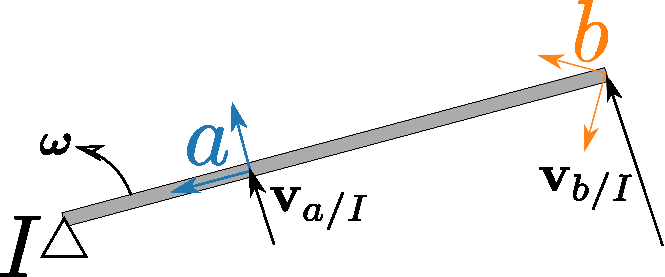
\includegraphics[width=0.3\columnwidth]{chap2_preliminaries/figures/rotating_bar}
\par\end{centering}
\caption{Illustration of a rotating rigid body with two coordinate frames.
The Adjoint of $\protect\SE\left(3\right)$ will convert $\protect\w$
and $\protect\v$ from frame $a$ to frame $b$, and account for the
change in translation. }
\label{fig:rotating_adjoint}
\end{figure}


\subsection{Adjoint of Dual Quaternions}

As with unit quaternions, dual unit quaternions are also self-adjoint:

\[
\Ad\left(\qq\right)=\qq\cdot\exp\left(\d\right)\cdot\qq^{-1}.
\]
We have no problem dealing with six-vectors here (the problem with
$\SE\left(3\right),$which led us to compute that hairy limit). However,
just like unit quaternions, we can compute the matrix form of the
Adjoint using the limit expression. Again, let's split up the generators
into two groups to help keep things a little more concise

{\small{}
\begin{align*}
\Ad_{1-3} & =\lim_{\varepsilon\to0}\frac{1}{\varepsilon}\begin{bmatrix}\log\left(\qq\cdot\exp\left(J_{1}\varepsilon\right)\cdot\qq^{-1}\right) & \cdots\end{bmatrix}\\
 & =\lim_{\varepsilon\to0}\frac{1}{\varepsilon}\begin{bmatrix}\log\left(\begin{bmatrix}\qbf_{r}\\
\epsilon\qbf_{d}
\end{bmatrix}\cdot\begin{bmatrix}\begin{pmatrix}0\\
\e_{1}\sin\left(\frac{\varepsilon}{2}\right)
\end{pmatrix}\\
0\epsilon
\end{bmatrix}\cdot\begin{bmatrix}\qbf_{r}\\
\epsilon\qbf_{d}
\end{bmatrix}^{-1}\right) & \cdots\end{bmatrix}\\
 & =\lim_{\varepsilon\to0}\frac{1}{\varepsilon}\begin{bmatrix}\log\left(\begin{bmatrix}\qbf_{r}\\
\epsilon\qbf_{d}
\end{bmatrix}\cdot\begin{bmatrix}\e_{1}\varepsilon\\
0\epsilon
\end{bmatrix}\cdot\begin{bmatrix}\qbf_{r}\\
\epsilon\qbf_{d}
\end{bmatrix}^{-1}\right) & \cdots\end{bmatrix} & \grey{\sin\varepsilon\to\varepsilon}\\
 & =\lim_{\varepsilon\to0}\frac{1}{\varepsilon}\begin{bmatrix}\log\left(\begin{bmatrix}\qbf_{r}\cdot\e_{1}^{\wedge}\varepsilon\\
\epsilon\left(\e_{1}^{\wedge}\varepsilon\cdot\qbf_{d}\right)
\end{bmatrix}\cdot\begin{bmatrix}\qbf_{r}\\
\epsilon\qbf_{d}
\end{bmatrix}^{-1}\right) & \cdots\end{bmatrix}\\
 & =\lim_{\varepsilon\to0}\frac{1}{\varepsilon}\begin{bmatrix}\log\left(\begin{bmatrix}\qbf_{r}\cdot\e_{1}^{\wedge}\varepsilon\cdot\qbf_{r}^{-1}\\
\epsilon\left(\qbf_{r}\cdot\e_{1}^{\wedge}\varepsilon\cdot\qbf_{d}^{-1}+\qbf_{r}^{-1}\cdot\e_{1}^{\wedge}\varepsilon\cdot\qbf_{d}\right)
\end{bmatrix}\right) & \cdots\end{bmatrix} & \grey{\e_{1}^{\wedge}=\begin{pmatrix}0\\
\e_{1}
\end{pmatrix}}\\
 & =\lim_{\varepsilon\to0}\frac{1}{\varepsilon}\begin{bmatrix}\log\left(\begin{bmatrix}\qbf_{r}\cdot\e_{1}^{\wedge}\varepsilon\cdot\qbf_{r}^{-1}\\
\epsilon\left(\qbf_{r}\cdot\e_{1}^{\wedge}\varepsilon\cdot\begin{pmatrix}\frac{1}{2}\t^{\wedge}\cdot\qbf_{r}\end{pmatrix}^{-1}+\qbf_{r}^{-1}\cdot\e_{1}^{\wedge}\varepsilon\cdot\frac{1}{2}\t^{\wedge}\cdot\qbf_{r}\right)
\end{bmatrix}\right) & \cdots\end{bmatrix}\\
 & =\lim_{\varepsilon\to0}\frac{1}{\varepsilon}\begin{bmatrix}\log\left(\begin{bmatrix}\qbf_{r}\cdot\e_{1}^{\wedge}\varepsilon\cdot\qbf_{r}^{-1}\\
\frac{1}{2}\epsilon\left(\qbf_{r}\cdot\e_{1}^{\wedge}\varepsilon\cdot\qbf_{r}^{-1}\cdot\left(-\t^{\wedge}\right)+\qbf_{r}^{-1}\cdot\e_{1}^{\wedge}\varepsilon\cdot\t^{\wedge}\cdot\qbf_{r}\right)
\end{bmatrix}\right) & \cdots\end{bmatrix}\\
 & =\lim_{\varepsilon\to0}\frac{1}{\varepsilon}\begin{bmatrix}\log\left(\begin{bmatrix}\qbf_{r}\cdot\e_{1}^{\wedge}\varepsilon\cdot\qbf_{r}^{-1}\\
\frac{1}{2}\epsilon\left(-\skew{R^{\top}\e_{1}\varepsilon}\t+R\skew{\e_{1}\varepsilon}\t\right)
\end{bmatrix}\right) & \cdots\end{bmatrix} & \grey{\textrm{(Eq. \ref{eq:quat_mult_matrix})}}\\
 & =\lim_{\varepsilon\to0}\frac{1}{\varepsilon}\begin{bmatrix}\log\left(\begin{bmatrix}\qbf_{r}\cdot\e_{1}^{\wedge}\varepsilon\cdot\qbf_{r}^{-1}\\
\frac{1}{2}\epsilon\left(-R^{\top}\skew{\e_{1}\varepsilon}R\t+R\skew{\e_{1}\varepsilon}\t\right)
\end{bmatrix}\right) & \cdots\end{bmatrix} & \grey{\textrm{(Eq. \ref{eq:skew_trick_2})}}\\
 & =\lim_{\varepsilon\to0}\frac{1}{\varepsilon}\begin{bmatrix}\log\left(\begin{bmatrix}\qbf_{r}\cdot\e_{1}^{\wedge}\varepsilon\cdot\qbf_{r}^{-1}\\
\frac{1}{2}\epsilon\left(R^{\top}\skew{R\t}\e_{1}\varepsilon-R\skew{\t}\e_{1}\varepsilon\right)
\end{bmatrix}\right) & \cdots\end{bmatrix} & \grey{\textrm{(Eq. \ref{eq:skew_trick_1})}}\\
 & =\lim_{\varepsilon\to0}\frac{1}{\varepsilon}\begin{bmatrix}\log\left(\begin{bmatrix}\qbf_{r}\cdot\e_{1}^{\wedge}\varepsilon\cdot\qbf_{r}^{-1}\\
\frac{1}{2}\epsilon\left(\skew{\t}R^{\top}\e_{1}\varepsilon-R\skew{\t}\e_{1}\varepsilon\right)
\end{bmatrix}\right) & \cdots\end{bmatrix} & \grey{\textrm{(Eq. \ref{eq:skew_trick_1})}}\\
 & =\begin{bmatrix}R^{\top}\\
\skew{\t}R^{\top}
\end{bmatrix}.
\end{align*}
Whew! Luckily, the translation generators are much easier:}{\small\par}

\begin{align*}
\Ad_{4-6} & =\lim_{\varepsilon\to0}\frac{1}{\varepsilon}\begin{bmatrix}\log\left(\qq\cdot\exp\left(J_{1}\varepsilon\right)\cdot\qq^{-1}\right) & \cdots\end{bmatrix}\\
 & =\lim_{\varepsilon\to0}\frac{1}{\varepsilon}\begin{bmatrix}\log\left(\begin{bmatrix}\qbf_{r}\\
\epsilon\qbf_{d}
\end{bmatrix}\cdot\begin{bmatrix}0\\
\e_{1}\epsilon
\end{bmatrix}\cdot\begin{bmatrix}\qbf_{r}\\
\epsilon\qbf_{d}
\end{bmatrix}^{-1}\right) & \cdots\end{bmatrix}\\
 & =\lim_{\varepsilon\to0}\frac{1}{\varepsilon}\begin{bmatrix}\log\left(\begin{bmatrix}0\\
\epsilon\left(\qbf_{r}\cdot\e_{q}\varepsilon\right)
\end{bmatrix}\cdot\begin{bmatrix}\qbf_{r}\\
\epsilon\qbf_{d}
\end{bmatrix}^{-1}\right) & \cdots\end{bmatrix}\\
 & =\lim_{\varepsilon\to0}\frac{1}{\varepsilon}\begin{bmatrix}\log\begin{bmatrix}0\\
\epsilon\left(\qbf_{r}\cdot\e_{q}\varepsilon\cdot\qbf_{r}^{-1}\right)
\end{bmatrix} & \cdots\end{bmatrix}\\
 & =\lim_{\varepsilon\to0}\frac{1}{\varepsilon}\begin{bmatrix}\log\begin{bmatrix}0\\
\epsilon\left(R^{\top}\e_{1}\varepsilon\right)
\end{bmatrix} & \cdots\end{bmatrix}\\
 & =R^{\top}.
\end{align*}
Finally, we can write the full Adjoint for dual quaternions as

\[
\boxed{\Ad\left(\qq\right)=\begin{pmatrix}R^{\top} & 0\\
\skew{\t}R^{\top} & R^{\top}
\end{pmatrix}},
\]
which, unsurprisingly, is the same as the Adjoint of $\SE\left(3\right)$,
except with all the rotations transposed (due to the reverse order
of quaternions rotation with respect to $\SO\left(3\right).$) Note
that this is also the matrix inverse of the Adjoint of $\SE\left(3\right)$. 

Now that we have each of the Adjoints, we can use the tables in Appendix
\ref{sec:Tables} to find Jacobians for almost any arbitrary expression
involving Lie groups!

\section{Left vs Right Jacobians}

For now, just read \cite{Sola2019}. They have a great discussion
on this topic. 

TL;DR: Most of the time, I end up using the left Jacobian. Depending
on how you define error, however, you may want to use the right Jacobian.
If things are still hazy after reading Sola, write unit tests of your
implementations and make sure everything is self-consistent.

\appendix

\section{Useful Tables}

\label{sec:Tables}

\begin{table}[H]
\centering{}\caption{Common dual number formulae}
\label{tab:dual_trig_functions}%
\noindent\ovalbox{\begin{minipage}[t]{1\columnwidth - 2\fboxsep - 0.8pt}%
\begin{center}
\begin{align*}
f\left(r+d\epsilon\right) & =f\left(r\right)+\epsilon d\left(f^{\prime}\left(r\right)\right)\\
\cos\left(r+d\epsilon\right) & =\cos r-\epsilon d\sin r\\
\sin\left(r+d\epsilon\right) & =\sin r+\epsilon d\cos r\\
\arctan\left(r+d\epsilon\right) & =\arctan r+\epsilon\frac{d}{r^{2}+1}\\
\left(r+d\epsilon\right)^{2} & =r^{2}+\epsilon2rd\\
\sqrt{r+d\epsilon} & =\sqrt{r}+\epsilon\frac{d}{2\sqrt{r}}
\end{align*}
\par\end{center}%
\end{minipage}}
\end{table}

\begin{table}[H]
\begin{centering}
\caption{Taylor series expansions}
\label{tab:taylor_series}
\par\end{centering}
\noindent\ovalbox{\begin{minipage}[t][1\totalheight][c]{1\columnwidth - 2\fboxsep - 0.8pt}%
\begin{align*}
\sin\left(\theta\right) & =\theta-\frac{1}{3!}\theta^{3}+\frac{1}{5!}\theta^{5}\cdots\\
\cos\left(\theta\right) & =1-\frac{1}{2}\theta^{2}+\frac{1}{4!}\theta^{4}\cdots\\
\cos\left(\frac{\theta}{2}\right) & =1-\frac{1}{8}\theta^{2}+\frac{1}{46080}\theta^{4}\cdots\\
\frac{\sin\left(\theta\right)}{\theta} & =1-\frac{1}{3!}\theta^{2}+\frac{1}{5!}\theta^{4}\cdots\\
\frac{\sin\left(\frac{\theta}{2}\right)}{\theta} & =\frac{1}{2}-\frac{1}{48}\theta^{2}+\frac{1}{3840}\theta^{4}+\cdots\\
\frac{\theta}{\sin\left(\theta\right)} & =1+\frac{1}{3!}\theta^{2}+\frac{7}{360}\theta^{4}\cdots\\
\frac{1-\cos\left(\theta\right)}{\theta^{2}} & =\frac{1}{2}-\frac{1}{24}\theta^{2}+\frac{1}{720}\theta^{4}\cdots\\
\frac{\cos\theta-\frac{\sin\theta}{\theta}}{\theta^{2}} & =-\frac{1}{3}+\frac{1}{30}\theta^{2}-\frac{1}{840}\theta^{4}\cdots\\
\frac{\frac{1}{2}\cos\frac{\theta}{2}-\frac{\sin\frac{\theta}{2}}{\theta}}{\theta^{2}} & =-\frac{1}{24}+\frac{1}{960}\theta^{2}-\frac{1}{107520}\theta^{4}\cdots\\
\frac{\tan^{-1}\left(\frac{\theta}{y}\right)}{\theta} & =\frac{1}{y}-\frac{1}{3y^{3}}\theta^{2}+\frac{1}{5y^{5}}\theta^{4}
\end{align*}
%
\end{minipage}}
\end{table}

\begin{table}[H]
\begin{centering}
\caption{Group-Group Jacobians}
\label{tab:lie_identities_group_operations}
\par\end{centering}
\noindent\ovalbox{\begin{minipage}[t][1\totalheight][c]{1\columnwidth - 2\fboxsep - 0.8pt}%
\begin{center}
\begin{tabular}{>{\centering}b{0.27\linewidth}>{\centering}b{0.27\linewidth}>{\centering}b{0.27\linewidth}}
\noalign{\vskip0.25cm}
Expression & Left Jacobian & Right Jacobian\tabularnewline
\hline 
\noalign{\vskip0.15cm}
$\frac{\partial}{\partial\x}\y\cdot\x$ & $\Ad\left(\y\right)^{-1}$ & $I$\tabularnewline[0.15cm]
\noalign{\vskip0.15cm}
$\frac{\partial}{\partial\x}\x^{-1}\cdot\y$ & $-\Ad\left(\x\right)^{-1}$ & $-\Ad\left(\x^{-1}\cdot\y\right)^{-1}$\tabularnewline[0.15cm]
\noalign{\vskip0.15cm}
$\frac{\partial}{\partial\x}\y\cdot\x^{-1}$ & $-\Ad\left(\y\cdot\x^{-1}\right)$ & $-\Ad\left(\x\right)$\tabularnewline[0.15cm]
\noalign{\vskip0.15cm}
$\frac{\partial}{\partial\x}\x\cdot\y$ & $I$ & $\Ad\left(\y\right)^{-1}$\tabularnewline[0.15cm]
\end{tabular}{\small{}
\begin{align*}
\x,\y & \in G
\end{align*}
}
\par\end{center}%
\end{minipage}}
\end{table}

\begin{table}[H]
\begin{centering}
\caption{Useful Jacobians for $\protect\SO\left(3\right)$}
\label{tab:lie_identities_group_vector_s03}
\par\end{centering}
\noindent\ovalbox{\begin{minipage}[t][1\totalheight][c]{1\columnwidth - 2\fboxsep - 0.8pt}%
\begin{center}
\begin{tabular}{>{\centering}b{0.27\linewidth}>{\centering}b{0.27\linewidth}>{\centering}b{0.27\linewidth}}
\noalign{\vskip0.25cm}
Expression & Left Jacobian & Right Jacobian\tabularnewline
\hline 
\noalign{\vskip0.15cm}
$\frac{\partial}{\partial\x}R\cdot\v$ & $-\skew{R\cdot\v}$ & $-R\cdot\skew{\v}$\tabularnewline[0.15cm]
\noalign{\vskip0.15cm}
$\frac{\partial}{\partial\x}R^{\top}\cdot\v$ & $R^{\top}\skew{\v}$ & $\skew{R^{\top}\cdot\v}$\tabularnewline[0.15cm]
\noalign{\vskip0.15cm}
$\frac{\partial}{\partial\w}\exp\left(\skew{\w}\right)$ & $aI+b\skew{\w}+c\w\w^{\top}$ & $aI-b\skew{\w}+c\w\w^{\top}$\tabularnewline[0.15cm]
\noalign{\vskip0.15cm}
$\frac{\partial}{\partial R}\log\left(R\right)$ & $I-\frac{1}{2}\skew{\dd}+e\skew{\dd}^{2}$ & $I+\frac{1}{2}\skew{\dd}+e\skew{\dd}^{2}$\tabularnewline[0.15cm]
\end{tabular}
\par\end{center}
\begin{center}
$R\in\SO\left(3\right),\quad\v,\w\in\mathbb{R}^{3}\quad\dd=\log\left(R\right)\quad\theta=\norm{\dd}$
\par\end{center}
\begin{center}
$a=\frac{\sin\theta}{\theta}\quad b=\frac{1-\cos\left(\theta\right)}{\theta^{2}}\quad c=\frac{1-a}{\theta^{2}}\quad e=\frac{b-2c}{2a}$
\par\end{center}%
\end{minipage}}
\end{table}

\begin{table}[H]
\begin{centering}
\caption{Useful Jacobians Jacobians for $\protect\SE\left(3\right)$}
\label{tab:lie_identities_group_vector-se3}
\par\end{centering}
\noindent\ovalbox{\begin{minipage}[t][1\totalheight][c]{1\columnwidth - 2\fboxsep - 0.8pt}%
\begin{center}
\begin{tabular}{>{\centering}b{0.17\linewidth}>{\centering}b{0.32\linewidth}>{\centering}b{0.32\linewidth}}
\noalign{\vskip0.25cm}
Expression & Left Jacobian & Right Jacobian\tabularnewline
\hline 
\noalign{\vskip0.15cm}
$\frac{\partial}{\partial\x}T\cdot\v$ & $\begin{pmatrix}-\skew{R\cdot\v+\t} & I\end{pmatrix}$ & $\begin{pmatrix}-R\cdot\skew{\v} & R\end{pmatrix}$\tabularnewline[0.15cm]
\noalign{\vskip0.15cm}
$\frac{\partial}{\partial\x}T^{-1}\cdot\v$ & $\begin{pmatrix}R^{\top}\cdot\skew{\v} & -R^{\top}\end{pmatrix}$ & $\begin{pmatrix}\skew{R^{\top}\cdot\left(\v-\t\right)} & -I\end{pmatrix}$\tabularnewline[0.15cm]
\noalign{\vskip0.15cm}
$\frac{\partial}{\partial\boldsymbol{\xi}}\exp\left(\boldsymbol{\xi}^{\wedge}\right)$ & $\begin{pmatrix}A & 0\\
D & A
\end{pmatrix}$ & $\begin{pmatrix}A^{\top} & 0\\
D^{\top} & A^{\top}
\end{pmatrix}$\tabularnewline[0.15cm]
\noalign{\vskip0.15cm}
$\frac{\partial}{\partial T}\log\left(T\right)$ & $\begin{pmatrix}E & 0\\
-E\cdot D\cdot E & E
\end{pmatrix}$ & $\begin{pmatrix}E^{\top} & 0\\
-\left(E\cdot D\cdot E\right)^{\top} & E^{\top}
\end{pmatrix}$\tabularnewline[0.15cm]
\end{tabular}
\par\end{center}
\begin{center}
$T\in\SE\left(3\right),\quad\v\in\mathbb{R}^{3},\quad\boldsymbol{\xi}=\begin{pmatrix}\w & \v\end{pmatrix}^{\top}\in\se\left(3\right)$
\par\end{center}
\begin{center}
$a=\frac{\sin\theta}{\theta}\quad b=\frac{1-\cos\left(\theta\right)}{\theta^{2}}\quad c=\frac{1-a}{\theta^{2}}\quad d=\w^{\top}\v\quad A=\frac{\partial}{\partial\w}\exp\left(\skew{\w}\right)$
\par\end{center}
\begin{center}
$B=\w\v^{\top}+\v\w^{\top}\quad C=\left(c-b\right)I+\left(\frac{a-2b}{\theta^{2}}\right)\skew{\w}+\left(\frac{b-3c}{\theta^{2}}\right)\w\w^{\top}$
\par\end{center}
\begin{center}
$D=b\skew{\v}+cB+dC\quad E=\frac{\partial}{\partial R}\log\left(R\right)$
\par\end{center}%
\end{minipage}}
\end{table}

\begin{table}[H]
\begin{centering}
\caption{Useful Jacobians for $\protect\S^{3}$}
\label{tab:lie_identities_s3}
\par\end{centering}
\noindent\ovalbox{\begin{minipage}[t][1\totalheight][c]{1\columnwidth - 2\fboxsep - 0.8pt}%
\begin{center}
\begin{tabular}{>{\centering}b{0.27\linewidth}>{\centering}b{0.27\linewidth}>{\centering}b{0.27\linewidth}}
\noalign{\vskip0.25cm}
Expression & Left Jacobian & Right Jacobian\tabularnewline
\hline 
\noalign{\vskip0.15cm}
$\frac{\partial}{\partial\x}\q^{-1}\cdot\v^{\wedge}\cdot\q$ & $R\left(\q\right)^{\top}\cdot\skew{\v}$ & $\skew{R\left(\q\right)^{\top}\cdot\v}$\tabularnewline[0.15cm]
\noalign{\vskip0.15cm}
$\frac{\partial}{\partial\x}\q\cdot\v^{\wedge}\cdot\q^{-1}$ & $-\skew{R\left(\q\right)}\cdot\v$ & $-R\left(\q\right)\cdot\skew{\v}$\tabularnewline[0.15cm]
\noalign{\vskip0.15cm}
$\frac{\partial}{\partial\w}\exp\left(\w^{\wedge}\right)$ & $aI+b\skew{\w}+c\w\w^{\top}$ & $aI-b\skew{\w}+c\w\w^{\top}$\tabularnewline[0.15cm]
\noalign{\vskip0.15cm}
$\frac{\partial}{\partial\q}\log\left(\q\right)$ & $I-\frac{1}{2}\skew{\dd}+e\skew{\dd}^{2}$ & $I+\frac{1}{2}\skew{\dd}+e\skew{\dd}^{2}$\tabularnewline[0.15cm]
\end{tabular}
\par\end{center}
\begin{center}
$\q\in\S^{3}\quad\v,\w\in\mathfrak{s}^{3}\quad\dd=\log\left(\q\right)\quad\theta=\norm{\dd}$\\
$a=\frac{\sin\theta}{\theta}\quad b=\frac{1-\cos\left(\theta\right)}{\theta^{2}}\quad c=\frac{1-a}{\theta^{2}}\quad e=\frac{b-2c}{2a}$
\par\end{center}%
\end{minipage}}
\end{table}

\begin{table}[H]
\begin{centering}
\caption{Useful Jacobians for $\mathbb{D}\protect\S^{3}$}
\label{tab:lie_identities_ds3}
\par\end{centering}
\noindent\ovalbox{\begin{minipage}[t][1\totalheight][c]{1\columnwidth - 2\fboxsep - 0.8pt}%
\begin{center}
\begin{tabular}{>{\centering}b{0.19\linewidth}>{\centering}b{0.31\linewidth}>{\centering}b{0.31\linewidth}}
\noalign{\vskip0.25cm}
Expression & Left Jacobian & Right Jacobian\tabularnewline
\hline 
\noalign{\vskip0.15cm}
$\frac{\partial}{\partial\x}\qq^{-1}\cdot\v^{\wedge}\cdot\qq$ & $\begin{pmatrix}R\left(\qbf_{r}\right)\skew{\v} & R\left(\q\right)\end{pmatrix}$ & $\begin{pmatrix}\skew{R\left(\qbf_{r}\right)\left(\v-\t\right)} & -I\end{pmatrix}$\tabularnewline[0.15cm]
\noalign{\vskip0.15cm}
$\frac{\partial}{\partial\x}\qq\cdot\v^{\wedge}\cdot\qq^{-1}$ & $\begin{pmatrix}-\skew{R\left(\qbf_{r}\right)^{\top}}\v+\t & I\end{pmatrix}$ & $\begin{pmatrix}R\left(\qbf_{r}\right)^{\top}\skew{-\v} & R\left(\qbf_{r}\right)^{\top}\end{pmatrix}$\tabularnewline[0.15cm]
\noalign{\vskip0.15cm}
$\frac{\partial}{\partial\boldsymbol{\xi}}\exp\left(\boldsymbol{\xi^{\wedge}}\right)$ & $\begin{pmatrix}A & 0\\
D & A
\end{pmatrix}$ & $\begin{pmatrix}A^{\top} & 0\\
D^{\top} & A^{\top}
\end{pmatrix}$\tabularnewline[0.15cm]
\noalign{\vskip0.15cm}
$\frac{\partial}{\partial T}\log\left(\qq\right)$ & $\begin{pmatrix}E & 0\\
-E\cdot D\cdot E & E
\end{pmatrix}$ & $\begin{pmatrix}E^{\top} & 0\\
\left(-E\cdot D\cdot E\right)^{\top} & E^{\top}
\end{pmatrix}$\tabularnewline[0.15cm]
\end{tabular}
\par\end{center}
\begin{center}
$\qq\in\mathbb{D}\S^{3},\quad\boldsymbol{\xi}=\begin{pmatrix}\w & \v\end{pmatrix}^{\top}\in\mathfrak{ds}^{3}$
\par\end{center}
\begin{center}
$a=\frac{\sin\theta}{\theta}\quad b=\frac{1-\cos\left(\theta\right)}{\theta^{2}}\quad c=\frac{1-a}{\theta^{2}}\quad d=\w^{\top}\v\quad A=\frac{\partial}{\partial\w}\exp\left(\skew{\w}\right)$
\par\end{center}
\begin{center}
$B=\w\v^{\top}+\v\w^{\top}\quad C=\left(c-b\right)I+\left(\frac{a-2b}{\theta^{2}}\right)\skew{\w}+\left(\frac{b-3c}{\theta^{2}}\right)\w\w^{\top}$
\par\end{center}
\begin{center}
$D=b\skew{\v}+cB+dC\quad E=\frac{\partial}{\partial R}\log\left(R\right)$
\par\end{center}%
\end{minipage}}
\end{table}

\bibliographystyle{plain}
\bibliography{library}

\end{document}
